\section{FMM3d\_\-MPI Class Reference}
\label{classFMM3d__MPI}\index{FMM3d_MPI@{FMM3d\_\-MPI}}
{\tt \#include $<$fmm3d\_\-mpi.hpp$>$}

Inheritance diagram for FMM3d\_\-MPI::\begin{figure}[H]
\begin{center}
\leavevmode
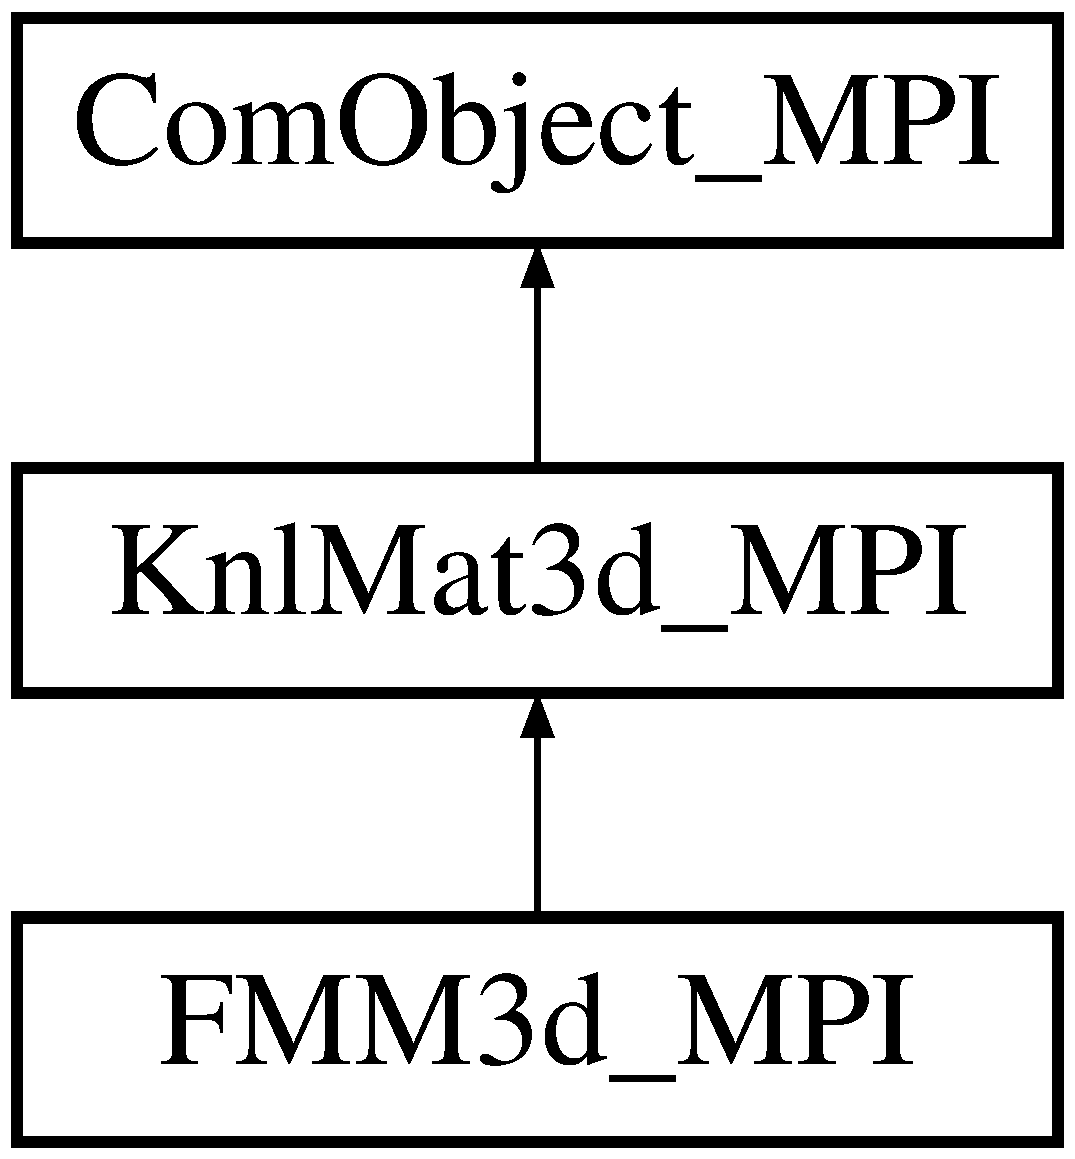
\includegraphics[height=3cm]{classFMM3d__MPI}
\end{center}
\end{figure}


\subsection{Detailed Description}
FMM3d\_\-MPI inherits from {\bf Knl\-Mat3d\_\-MPI}{\rm (p.\,\pageref{classKnlMat3d__MPI})}. Specific information for computing and using FMM are implemented here. Specifically, setup and evaluate and inherits source positions, etc. See {\bf knlmat3d\_\-mpi.hpp}{\rm (p.\,\pageref{knlmat3d__mpi_8hpp})} for more information. 



Definition at line 36 of file fmm3d\_\-mpi.hpp.\subsection*{Public Types}
\begin{CompactItemize}
\item 
typedef pair$<$ int, int $>$ {\bf intpair}
\item 
enum \{ {\bf UE} = 0, 
{\bf UC} = 1, 
{\bf DE} = 2, 
{\bf DC} = 3
 \}
\end{CompactItemize}
\subsection*{Public Member Functions}
\begin{CompactItemize}
\item 
{\bf FMM3d\_\-MPI} (const string \&p)
\item 
{\bf $\sim$FMM3d\_\-MPI} ()
\item 
Point3 \& {\bf ctr} ()
\item 
int \& {\bf root\-Level} ()
\item 
int \& {\bf np} ()
\item 
int {\bf setup} ()
\item 
int {\bf evaluate} (Vec src\-Den, Vec trg\-Val)
\item 
int {\bf check} (Vec src\-Den, Vec trg\-Val, int numchk, double \&rerr)
\item 
{\bf Let3d\_\-MPI} $\ast$ {\bf let} ()
\item 
{\bf Mat\-Mgnt3d\_\-MPI} $\ast$ {\bf matmgnt} ()
\item 
{\bf Node} \& {\bf node} (int g\-Node\-Idx)
\end{CompactItemize}
\subsection*{Protected Member Functions}
\begin{CompactItemize}
\item 
int {\bf dat\-Sze} (int tp)
\item 
int {\bf Src\-Equ2Trg\-Chk\_\-dgemv} (const Dbl\-Num\-Mat \&src\-Pos, const Dbl\-Num\-Mat \&src\-Nor, const Dbl\-Num\-Mat \&trg\-Pos, const Dbl\-Num\-Vec \&src\-Den, Dbl\-Num\-Vec \&trg\-Val)
\item 
int {\bf Src\-Equ2Upw\-Chk\_\-dgemv} (const Dbl\-Num\-Mat \&src\-Pos, const Dbl\-Num\-Mat \&src\-Nor, Point3 trgctr, double trgrad, const Dbl\-Num\-Vec \&src\-Den, Dbl\-Num\-Vec \&trg\-Val)
\item 
int {\bf Src\-Equ2Dwn\-Chk\_\-dgemv} (const Dbl\-Num\-Mat \&src\-Pos, const Dbl\-Num\-Mat \&src\-Nor, Point3 trgctr, double trgrad, const Dbl\-Num\-Vec \&src\-Den, Dbl\-Num\-Vec \&trg\-Val)
\item 
int {\bf Dwn\-Equ2Trg\-Chk\_\-dgemv} (Point3 srcctr, double srcrad, const Dbl\-Num\-Mat \&trg\-Pos, const Dbl\-Num\-Vec \&src\-Den, Dbl\-Num\-Vec \&trg\-Val)
\item 
int {\bf Upw\-Equ2Trg\-Chk\_\-dgemv} (Point3 srcctr, double srcrad, const Dbl\-Num\-Mat \&trg\-Pos, const Dbl\-Num\-Vec \&src\-Den, Dbl\-Num\-Vec \&trg\-Val)
\item 
Dbl\-Num\-Mat {\bf ctb\-Src\-Exa\-Pos} (int g\-Node\-Idx)
\item 
Dbl\-Num\-Mat {\bf ctb\-Src\-Exa\-Nor} (int g\-Node\-Idx)
\item 
Dbl\-Num\-Vec {\bf ctb\-Src\-Exa\-Den} (int g\-Node\-Idx)
\item 
Dbl\-Num\-Vec {\bf ctb\-Src\-Upw\-Equ\-Den} (int g\-Node\-Idx)
\item 
Dbl\-Num\-Vec {\bf ctb\-Src\-Upw\-Chk\-Val} (int g\-Node\-Idx)
\item 
Dbl\-Num\-Mat {\bf usr\-Src\-Exa\-Pos} (int g\-Node\-Idx)
\item 
Dbl\-Num\-Mat {\bf usr\-Src\-Exa\-Nor} (int g\-Node\-Idx)
\item 
Dbl\-Num\-Vec {\bf usr\-Src\-Exa\-Den} (int g\-Node\-Idx)
\item 
Dbl\-Num\-Vec {\bf usr\-Src\-Upw\-Equ\-Den} (int g\-Node\-Idx)
\item 
Dbl\-Num\-Mat {\bf eva\-Trg\-Exa\-Pos} (int g\-Node\-Idx)
\item 
Dbl\-Num\-Vec {\bf eva\-Trg\-Exa\-Val} (int g\-Node\-Idx)
\item 
Dbl\-Num\-Vec {\bf eva\-Trg\-Dwn\-Equ\-Den} (int g\-Node\-Idx)
\item 
Dbl\-Num\-Vec {\bf eva\-Trg\-Dwn\-Chk\-Val} (int g\-Node\-Idx)
\end{CompactItemize}
\subsection*{Protected Attributes}
\begin{CompactItemize}
\item 
Point3 {\bf \_\-ctr}
\item 
int {\bf \_\-root\-Level}
\item 
int {\bf \_\-np}
\item 
{\bf Let3d\_\-MPI} $\ast$ {\bf \_\-let}
\item 
{\bf Mat\-Mgnt3d\_\-MPI} $\ast$ {\bf \_\-matmgnt}
\item 
vector$<$ {\bf Node} $>$ {\bf \_\-node\-Vec}
\item 
Vec {\bf \_\-glb\-Src\-Exa\-Pos}
\item 
Vec {\bf \_\-glb\-Src\-Exa\-Nor}
\item 
Vec {\bf \_\-glb\-Src\-Exa\-Den}
\item 
Vec {\bf \_\-glb\-Src\-Upw\-Equ\-Den}
\item 
Vec {\bf \_\-ctb\-Src\-Exa\-Pos}
\item 
Vec {\bf \_\-ctb\-Src\-Exa\-Nor}
\item 
Vec {\bf \_\-ctb\-Src\-Exa\-Den}
\item 
Vec {\bf \_\-ctb\-Src\-Upw\-Equ\-Den}
\item 
Vec {\bf \_\-ctb\-Src\-Upw\-Chk\-Val}
\item 
Vec\-Scatter {\bf \_\-ctb2Glb\-Src\-Exa\-Pos}
\item 
Vec\-Scatter {\bf \_\-ctb2Glb\-Src\-Exa\-Den}
\item 
Vec\-Scatter {\bf \_\-ctb2Glb\-Src\-Upw\-Equ\-Den}
\item 
Vec {\bf \_\-eva\-Trg\-Exa\-Pos}
\item 
Vec {\bf \_\-eva\-Trg\-Exa\-Val}
\item 
Vec {\bf \_\-eva\-Trg\-Dwn\-Equ\-Den}
\item 
Vec {\bf \_\-eva\-Trg\-Dwn\-Chk\-Val}
\item 
Vec {\bf \_\-usr\-Src\-Exa\-Pos}
\item 
Vec {\bf \_\-usr\-Src\-Exa\-Nor}
\item 
Vec {\bf \_\-usr\-Src\-Exa\-Den}
\item 
Vec {\bf \_\-usr\-Src\-Upw\-Equ\-Den}
\item 
Vec\-Scatter {\bf \_\-usr2Glb\-Src\-Exa\-Pos}
\item 
Vec\-Scatter {\bf \_\-usr2Glb\-Src\-Exa\-Den}
\item 
Vec\-Scatter {\bf \_\-usr2Glb\-Src\-Upw\-Equ\-Den}
\item 
{\bf Kernel3d\_\-MPI} {\bf \_\-knl\_\-mm}
\end{CompactItemize}
\subsection*{Classes}
\begin{CompactItemize}
\item 
class {\bf Node}
\begin{CompactList}\small\item\em {\bf Node}{\rm (p.\,\pageref{classFMM3d__MPI_1_1Node})} class for {\bf FMM3d\_\-MPI}{\rm (p.\,\pageref{classFMM3d__MPI})} stores access functions to {\bf Node\-Ext}{\rm (p.\,\pageref{classFMM3d__MPI_1_1NodeExt})}. \item\end{CompactList}\item 
class {\bf Node\-Ext}
\begin{CompactList}\small\item\em Extra node information. Different from {\bf Let3d\_\-MPI::Node\-Ext}{\rm (p.\,\pageref{classLet3d__MPI_1_1NodeExt})}. \item\end{CompactList}\end{CompactItemize}


\subsection{Member Typedef Documentation}
\index{FMM3d_MPI@{FMM3d\_\-MPI}!intpair@{intpair}}
\index{intpair@{intpair}!FMM3d_MPI@{FMM3d\_\-MPI}}
\subsubsection{\setlength{\rightskip}{0pt plus 5cm}typedef pair$<$int,int$>$ {\bf FMM3d\_\-MPI::intpair}}\label{classFMM3d__MPI_516fcca2e14cd2e14fd71db54824f696_516fcca2e14cd2e14fd71db54824f696}




Definition at line 39 of file fmm3d\_\-mpi.hpp.

\subsection{Member Enumeration Documentation}
\subsubsection{\setlength{\rightskip}{0pt plus 5cm}anonymous enum}\label{classFMM3d__MPI_dca29a1140aadadfd92b34a02fa516ef_dca29a1140aadadfd92b34a02fa516ef}


\begin{Desc}
\item[Enumerator: ]\par
\begin{description}
\index{UE@{UE}!FMM3d_MPI@{FMM3d\_\-MPI}}\index{FMM3d_MPI@{FMM3d\_\-MPI}!UE@{UE}}\item[{\em 
UE\label{classFMM3d__MPI_dca29a1140aadadfd92b34a02fa516ef_dca29a1140aadadfd92b34a02fa516ef0612e93d65abcdaeed533a0876474251}
}]Upward Equivalent \index{UC@{UC}!FMM3d_MPI@{FMM3d\_\-MPI}}\index{FMM3d_MPI@{FMM3d\_\-MPI}!UC@{UC}}\item[{\em 
UC\label{classFMM3d__MPI_dca29a1140aadadfd92b34a02fa516ef_dca29a1140aadadfd92b34a02fa516ef6a2fb30a2dacdda4d74122697262a8b7}
}]Upward Check \index{DE@{DE}!FMM3d_MPI@{FMM3d\_\-MPI}}\index{FMM3d_MPI@{FMM3d\_\-MPI}!DE@{DE}}\item[{\em 
DE\label{classFMM3d__MPI_dca29a1140aadadfd92b34a02fa516ef_dca29a1140aadadfd92b34a02fa516ef3a52f3c22ed6fcde5bf696a6c02c9e73}
}]Downward Equivalent \index{DC@{DC}!FMM3d_MPI@{FMM3d\_\-MPI}}\index{FMM3d_MPI@{FMM3d\_\-MPI}!DC@{DC}}\item[{\em 
DC\label{classFMM3d__MPI_dca29a1140aadadfd92b34a02fa516ef_dca29a1140aadadfd92b34a02fa516efcf75e54791dd1f49f918345fdfe2430b}
}]Downward Check \end{description}
\end{Desc}



Definition at line 40 of file fmm3d\_\-mpi.hpp.

\footnotesize\begin{verbatim}40        {          UE=0, UC=1, DE=2, DC=3,  };
\end{verbatim}\normalsize 




\subsection{Constructor \& Destructor Documentation}
\index{FMM3d_MPI@{FMM3d\_\-MPI}!FMM3d_MPI@{FMM3d\_\-MPI}}
\index{FMM3d_MPI@{FMM3d\_\-MPI}!FMM3d_MPI@{FMM3d\_\-MPI}}
\subsubsection{\setlength{\rightskip}{0pt plus 5cm}FMM3d\_\-MPI::FMM3d\_\-MPI (const string \& {\em p})}\label{classFMM3d__MPI_9f48ad5b4ec95878d1bb32a181525789_9f48ad5b4ec95878d1bb32a181525789}


Initialize FMM3d\_\-MPI with string. Calls constructor from {\bf Knl\-Mat3d\_\-MPI}{\rm (p.\,\pageref{classKnlMat3d__MPI})}, and initializes are vectors here to NULL and values to zero. Center defaults to (0,0,0), root\-Level to 0, and np to 6 

Definition at line 31 of file fmm3d\_\-mpi.cpp.

\footnotesize\begin{verbatim}31                                    :
32   KnlMat3d_MPI(p), _ctr(0,0,0), _rootLevel(0),
33   _np(6),
34   _let(NULL), _matmgnt(NULL),
35   _glbSrcExaPos(NULL), _glbSrcExaNor(NULL), _glbSrcExaDen(NULL), _glbSrcUpwEquDen(NULL),
36   _ctbSrcExaPos(NULL), _ctbSrcExaNor(NULL), _ctbSrcExaDen(NULL), _ctbSrcUpwEquDen(NULL),
37   _ctbSrcUpwChkVal(NULL), _ctb2GlbSrcExaPos(NULL), _ctb2GlbSrcExaDen(NULL), _ctb2GlbSrcUpwEquDen(NULL),
38   _evaTrgExaPos(NULL), _evaTrgExaVal(NULL), _evaTrgDwnEquDen(NULL), _evaTrgDwnChkVal(NULL),
39   _usrSrcExaPos(NULL), _usrSrcExaNor(NULL), _usrSrcExaDen(NULL), _usrSrcUpwEquDen(NULL),
40   _usr2GlbSrcExaPos(NULL), _usr2GlbSrcExaDen(NULL), _usr2GlbSrcUpwEquDen(NULL)
41 {
42 }

\end{verbatim}\normalsize 


\index{FMM3d_MPI@{FMM3d\_\-MPI}!~FMM3d_MPI@{$\sim$FMM3d\_\-MPI}}
\index{~FMM3d_MPI@{$\sim$FMM3d\_\-MPI}!FMM3d_MPI@{FMM3d\_\-MPI}}
\subsubsection{\setlength{\rightskip}{0pt plus 5cm}FMM3d\_\-MPI::$\sim$FMM3d\_\-MPI ()}\label{classFMM3d__MPI_2cb06cc1c18cba63ed0226e5e691b3ca_2cb06cc1c18cba63ed0226e5e691b3ca}




Definition at line 45 of file fmm3d\_\-mpi.cpp.

References \_\-glb\-Src\-Exa\-Nor, \_\-glb\-Src\-Exa\-Pos, and \_\-let.

\footnotesize\begin{verbatim}46 {
47   if(_let!=NULL)         delete _let;
48   
49   if(_glbSrcExaPos!=NULL) { iC( VecDestroy(_glbSrcExaPos) ); _glbSrcExaPos=NULL; }
50   if(_glbSrcExaNor!=NULL) { iC( VecDestroy(_glbSrcExaNor) ); _glbSrcExaPos=NULL; }
51   if(_glbSrcExaDen!=NULL) { iC( VecDestroy(_glbSrcExaDen) ); _glbSrcExaDen=NULL; }
52   if(_glbSrcUpwEquDen!=NULL) { iC( VecDestroy(_glbSrcUpwEquDen) ); _glbSrcUpwEquDen=NULL; }
53   
54   if(_ctbSrcExaPos!=NULL) { iC( VecDestroy(_ctbSrcExaPos) ); _ctbSrcExaPos=NULL; }
55   if(_ctbSrcExaNor!=NULL) { iC( VecDestroy(_ctbSrcExaNor) ); _ctbSrcExaNor=NULL; }
56   if(_ctbSrcExaDen!=NULL) { iC( VecDestroy(_ctbSrcExaDen) ); _ctbSrcExaDen=NULL; }
57   if(_ctbSrcUpwEquDen!=NULL) { iC( VecDestroy(_ctbSrcUpwEquDen) ); _ctbSrcUpwEquDen=NULL; }
58   if(_ctbSrcUpwChkVal!=NULL) { iC( VecDestroy(_ctbSrcUpwChkVal) ); _ctbSrcUpwChkVal=NULL; }
59   if(_ctb2GlbSrcExaPos!=NULL) { iC( VecScatterDestroy(_ctb2GlbSrcExaPos) ); _ctb2GlbSrcExaPos=NULL; }
60   if(_ctb2GlbSrcExaDen!=NULL) { iC( VecScatterDestroy(_ctb2GlbSrcExaDen) ); _ctb2GlbSrcExaDen=NULL; }
61   if(_ctb2GlbSrcUpwEquDen!=NULL) { iC( VecScatterDestroy(_ctb2GlbSrcUpwEquDen) ); _ctb2GlbSrcUpwEquDen=NULL; }
62   
63   if(_evaTrgExaPos!=NULL) { iC( VecDestroy(_evaTrgExaPos) ); _evaTrgExaPos=NULL; }
64   if(_evaTrgExaVal!=NULL) { iC( VecDestroy(_evaTrgExaVal) ); _evaTrgExaVal=NULL; }
65   if(_evaTrgDwnEquDen!=NULL) { iC( VecDestroy(_evaTrgDwnEquDen) ); _evaTrgDwnEquDen=NULL; }
66   if(_evaTrgDwnChkVal!=NULL) { iC( VecDestroy(_evaTrgDwnChkVal) ); _evaTrgDwnChkVal=NULL; }
67   
68   if(_usrSrcExaPos!=NULL) { iC( VecDestroy(_usrSrcExaPos) ); _usrSrcExaPos=NULL; }
69   if(_usrSrcExaNor!=NULL) { iC( VecDestroy(_usrSrcExaNor) ); _usrSrcExaNor=NULL; }
70   if(_usrSrcExaDen!=NULL) { iC( VecDestroy(_usrSrcExaDen) ); _usrSrcExaDen=NULL; }
71   if(_usrSrcUpwEquDen!=NULL) { iC( VecDestroy(_usrSrcUpwEquDen) ); _usrSrcUpwEquDen=NULL; }
72   if(_usr2GlbSrcExaPos!=NULL) { iC( VecScatterDestroy(_usr2GlbSrcExaPos) ); _usr2GlbSrcExaPos=NULL; }
73   if(_usr2GlbSrcExaDen!=NULL) { iC( VecScatterDestroy(_usr2GlbSrcExaDen) ); _usr2GlbSrcExaDen=NULL; }
74   if(_usr2GlbSrcUpwEquDen!=NULL) { iC( VecScatterDestroy(_usr2GlbSrcUpwEquDen) ); _usr2GlbSrcUpwEquDen=NULL; }
75 }
\end{verbatim}\normalsize 




\subsection{Member Function Documentation}
\index{FMM3d_MPI@{FMM3d\_\-MPI}!check@{check}}
\index{check@{check}!FMM3d_MPI@{FMM3d\_\-MPI}}
\subsubsection{\setlength{\rightskip}{0pt plus 5cm}int FMM3d\_\-MPI::check (Vec {\em src\-Den}, Vec {\em trg\-Val}, int {\em numchk}, double \& {\em rerr})}\label{classFMM3d__MPI_d2aa9de21b49559ceb1eb86a90536758_d2aa9de21b49559ceb1eb86a90536758}


check function, returns relative error. Detailed in fmm3d\_\-mpi\_\-check.cpp 

Definition at line 34 of file fmm3d\_\-check\_\-mpi.cpp.

References Knl\-Mat3d\_\-MPI::\_\-src\-Pos, Knl\-Mat3d\_\-MPI::\_\-trg\-Pos, Knl\-Mat3d\_\-MPI::dim(), Com\-Object\_\-MPI::mpi\-Size(), p\-A, Knl\-Mat3d\_\-MPI::proc\-Lcl\-Num(), Knl\-Mat3d\_\-MPI::src\-DOF(), and Knl\-Mat3d\_\-MPI::trg\-DOF().

\footnotesize\begin{verbatim}35 {
36   //begin
37   pA(procLclNum(_trgPos)>0); //have things to check
38   //pC( PetscPrintf(mpiComm(), "checking.........\n") );
39   int dim = this->dim();
40   int srcDOF = this->srcDOF();
41   int trgDOF = this->trgDOF();
42   int slclnum = procLclNum(_srcPos);
43   int tlclnum = procLclNum(_trgPos);   //int lclnum = this->lclnum();
44   
45   //1. select point to check
46   int ttlChk = numChk*mpiSize();
47   vector<int> chkVec(numChk);
48   for(int k=0; k<numChk; k++) {
49          chkVec[k] = int( floor(drand48()*tlclnum) );
50          pA(chkVec[k]>=0 && chkVec[k]<tlclnum);
51   }
52   pC( MPI_Barrier(mpiComm()) );
53   
54   Vec chkPos; pC( VecCreateMPI(mpiComm(), numChk*dim,  ttlChk*dim,  &chkPos) ); //check position
55   Vec chkVal; pC( VecCreateMPI(mpiComm(), numChk*trgDOF, ttlChk*trgDOF, &chkVal) ); //check value
56   Vec chkDen; pC( VecCreateMPI(mpiComm(), numChk*trgDOF, ttlChk*trgDOF, &chkDen) ); //check density
57   
58   double* posArr; pC( VecGetArray(_trgPos, &posArr) );
59   double* valArr; pC( VecGetArray( trgVal, &valArr) );
60   double* chkPosArr; pC( VecGetArray(chkPos, &chkPosArr) );
61   double* chkValArr; pC( VecGetArray(chkVal, &chkValArr) );
62   for(int k=0; k<numChk; k++) {
63          for(int i=0; i<dim; i++)
64                 chkPosArr[ k*dim+i  ] = posArr[ chkVec[k]*dim+i  ];
65          for(int i=0; i<trgDOF;i++)
66                 chkValArr[ k*trgDOF+i ] = valArr[ chkVec[k]*trgDOF+i ];
67   } 
68   pC( VecRestoreArray(_trgPos, &posArr) );
69   pC( VecRestoreArray( trgVal, &valArr) );
70   pC( VecRestoreArray(chkPos, &chkPosArr) );
71   pC( VecRestoreArray(chkVal, &chkValArr) );
72   
73   //2. compute and gather
74   Vec allChkPos;
75   {
76          VecScatter ctx;  pC( VecScatterCreateToAll(chkPos, &ctx, &allChkPos) );
77          pC( VecScatterBegin(chkPos, allChkPos, INSERT_VALUES, SCATTER_FORWARD, ctx) );
78          pC( VecScatterEnd(  chkPos, allChkPos, INSERT_VALUES, SCATTER_FORWARD, ctx) );
79          pC( VecScatterDestroy(ctx) );
80   }
81   Vec allChkDen; pC( VecCreateSeq(PETSC_COMM_SELF, ttlChk*trgDOF, &allChkDen) );
82   Vec glbChkDen; pC( VecCreateSeq(PETSC_COMM_SELF, ttlChk*trgDOF, &glbChkDen) );
83   
84   double* lclSrcPosArr; pC( VecGetArray(_srcPos, &lclSrcPosArr) );
85   double* lclSrcNorArr; pC( VecGetArray(_srcNor, &lclSrcNorArr) );
86   double* lclSrcDenArr; pC( VecGetArray( srcDen, &lclSrcDenArr) );
87   double* allChkPosArr; pC( VecGetArray(allChkPos, &allChkPosArr) );
88   double* allChkDenArr; pC( VecGetArray(allChkDen, &allChkDenArr) );
89   double* glbChkDenArr; pC( VecGetArray(glbChkDen, &glbChkDenArr) );
90   
91   DblNumMat lclSrcPosMat(dim, slclnum, false, lclSrcPosArr);
92   DblNumMat lclSrcNorMat(dim, slclnum, false, lclSrcNorArr);
93   DblNumVec lclSrcDenVec(srcDOF*slclnum, false, lclSrcDenArr);
94   DblNumMat allChkPosMat(dim,  ttlChk, false, allChkPosArr);
95   DblNumVec allChkDenVec(trgDOF* ttlChk, false, allChkDenArr);
96   
97   DblNumMat inter(trgDOF, slclnum*srcDOF);
98   for(int i=0; i<ttlChk; i++) {
99          DblNumMat oneChkPosMat(dim, 1, false, allChkPosMat.clmdata(i));
100          DblNumVec oneChkDenVec(trgDOF, false, allChkDenVec.data()+i*trgDOF);
101          pC( _knl.buildKnlIntCtx(lclSrcPosMat, lclSrcNorMat, oneChkPosMat, inter) );
102          pC( dgemv(1.0, inter, lclSrcDenVec, 0.0, oneChkDenVec) );
103   }
104   
105   pC( MPI_Barrier(mpiComm()) );
106   pC( MPI_Allreduce(allChkDenArr, glbChkDenArr, ttlChk*trgDOF, MPI_DOUBLE, MPI_SUM, mpiComm()) );
107   
108   //3. distribute to individual
109   double* lclChkDenArr; pC( VecGetArray(chkDen, &lclChkDenArr) );
110   void* dst = (void*)lclChkDenArr;
111   void* src = (void*)(glbChkDenArr + mpiRank()*numChk*trgDOF);  
112   memcpy(dst, src, sizeof(double)*numChk*trgDOF);
113   pC( VecRestoreArray(chkDen, &lclChkDenArr) );
114   
115   pC( VecRestoreArray(_srcPos, &lclSrcPosArr) );
116   pC( VecRestoreArray(_srcNor, &lclSrcNorArr) );
117   pC( VecRestoreArray( srcDen, &lclSrcDenArr) );
118   pC( VecRestoreArray(allChkPos, &allChkPosArr) );
119   pC( VecRestoreArray(allChkDen, &allChkDenArr) );
120   pC( VecRestoreArray(glbChkDen, &glbChkDenArr) );
121   
122   pC( VecDestroy(allChkPos) );
123   pC( VecDestroy(allChkDen) );
124   pC( VecDestroy(glbChkDen) );
125   
126   PetscScalar mone = -1.0;
127   pC( VecAXPY(chkVal, mone, chkDen) ); //chkVal now is the error - HARPER:  In correct order??
128   double nerr, npot;
129   pC( VecNorm(chkVal, NORM_2, &nerr) );
130   pC( VecNorm(chkDen, NORM_2, &npot) );
131   
132   rerr = nerr/npot;//pC( PetscPrintf(mpiComm(), "Error %e, %e %e\n", nerr/npot, nerr, npot) );
133   
134   pC( VecDestroy(chkPos) );
135   pC( VecDestroy(chkVal) );
136   pC( VecDestroy(chkDen) );
137   
138   return(0);
139 }
\end{verbatim}\normalsize 


\index{FMM3d_MPI@{FMM3d\_\-MPI}!ctbSrcExaDen@{ctbSrcExaDen}}
\index{ctbSrcExaDen@{ctbSrcExaDen}!FMM3d_MPI@{FMM3d\_\-MPI}}
\subsubsection{\setlength{\rightskip}{0pt plus 5cm}Dbl\-Num\-Vec FMM3d\_\-MPI::ctb\-Src\-Exa\-Den (int {\em g\-Node\-Idx})\hspace{0.3cm}{\tt  [protected]}}\label{classFMM3d__MPI_99138c2857a67a0f74ce4f752045aab1_99138c2857a67a0f74ce4f752045aab1}


Return vector of contributor exact source densities for a specific node - gets information from \_\-let 

Definition at line 273 of file fmm3d\_\-mpi.cpp.

References \_\-ctb\-Src\-Exa\-Den, \_\-let, Let3d\_\-MPI::Node::ctb\-Src\-Exa\-Beg(), Let3d\_\-MPI::Node::ctb\-Src\-Exa\-Num(), Let3d\_\-MPI::node(), node(), and Knl\-Mat3d\_\-MPI::src\-DOF().

Referenced by evaluate().

\footnotesize\begin{verbatim}274 {
275   Let3d_MPI::Node& node = _let->node(gNodeIdx);
276   int beg = node.ctbSrcExaBeg();
277   int num = node.ctbSrcExaNum();
278   double* arr;     VecGetArray(    _ctbSrcExaDen, &arr);
279   double* buf=arr; VecRestoreArray(_ctbSrcExaDen, &arr);
280   return DblNumVec(srcDOF()*num, false, buf+beg*srcDOF());
281 }
\end{verbatim}\normalsize 


\index{FMM3d_MPI@{FMM3d\_\-MPI}!ctbSrcExaNor@{ctbSrcExaNor}}
\index{ctbSrcExaNor@{ctbSrcExaNor}!FMM3d_MPI@{FMM3d\_\-MPI}}
\subsubsection{\setlength{\rightskip}{0pt plus 5cm}Dbl\-Num\-Mat FMM3d\_\-MPI::ctb\-Src\-Exa\-Nor (int {\em g\-Node\-Idx})\hspace{0.3cm}{\tt  [protected]}}\label{classFMM3d__MPI_3a82dc41a519275dec89995113a38cf3_3a82dc41a519275dec89995113a38cf3}


Return matrix of contributor exact source normals for a specific node - gets information from \_\-let 

Definition at line 263 of file fmm3d\_\-mpi.cpp.

References \_\-ctb\-Src\-Exa\-Nor, \_\-let, Let3d\_\-MPI::Node::ctb\-Src\-Exa\-Beg(), Let3d\_\-MPI::Node::ctb\-Src\-Exa\-Num(), Knl\-Mat3d\_\-MPI::dim(), Let3d\_\-MPI::node(), and node().

\footnotesize\begin{verbatim}264 {
265   Let3d_MPI::Node& node = _let->node(gNodeIdx);
266   int beg = node.ctbSrcExaBeg();
267   int num = node.ctbSrcExaNum();
268   double* arr;     VecGetArray(    _ctbSrcExaNor, &arr);
269   double* buf=arr; VecRestoreArray(_ctbSrcExaNor, &arr);
270   return DblNumMat(dim(), num, false, buf+beg*dim());
271 }
\end{verbatim}\normalsize 


\index{FMM3d_MPI@{FMM3d\_\-MPI}!ctbSrcExaPos@{ctbSrcExaPos}}
\index{ctbSrcExaPos@{ctbSrcExaPos}!FMM3d_MPI@{FMM3d\_\-MPI}}
\subsubsection{\setlength{\rightskip}{0pt plus 5cm}Dbl\-Num\-Mat FMM3d\_\-MPI::ctb\-Src\-Exa\-Pos (int {\em g\-Node\-Idx})\hspace{0.3cm}{\tt  [protected]}}\label{classFMM3d__MPI_5f4337de8f526dee009dc39c7c3213a6_5f4337de8f526dee009dc39c7c3213a6}


Return matrix of contributor exact source positions for a specific node - gets information from \_\-let 

Definition at line 253 of file fmm3d\_\-mpi.cpp.

References Let3d\_\-MPI::Node::ctb\-Src\-Exa\-Beg(), and Let3d\_\-MPI::Node::ctb\-Src\-Exa\-Num().

\footnotesize\begin{verbatim}254 {
255   Let3d_MPI::Node& node = _let->node(gNodeIdx);
256   int beg = node.ctbSrcExaBeg();
257   int num = node.ctbSrcExaNum();
258   double* arr;     VecGetArray(    _ctbSrcExaPos, &arr);
259   double* buf=arr; VecRestoreArray(_ctbSrcExaPos, &arr);
260   return DblNumMat(dim(), num, false, buf+beg*dim());
261 }
\end{verbatim}\normalsize 


\index{FMM3d_MPI@{FMM3d\_\-MPI}!ctbSrcUpwChkVal@{ctbSrcUpwChkVal}}
\index{ctbSrcUpwChkVal@{ctbSrcUpwChkVal}!FMM3d_MPI@{FMM3d\_\-MPI}}
\subsubsection{\setlength{\rightskip}{0pt plus 5cm}Dbl\-Num\-Vec FMM3d\_\-MPI::ctb\-Src\-Upw\-Chk\-Val (int {\em g\-Node\-Idx})\hspace{0.3cm}{\tt  [protected]}}\label{classFMM3d__MPI_db4b073fb62e65e5c0a52a3bcfe512c1_db4b073fb62e65e5c0a52a3bcfe512c1}


Return vector of contributor source upward check values for a specific node - gets information from \_\-let 

Definition at line 292 of file fmm3d\_\-mpi.cpp.

References \_\-ctb\-Src\-Upw\-Chk\-Val, \_\-let, Let3d\_\-MPI::Node::ctb\-Src\-Node\-Idx(), dat\-Sze(), Let3d\_\-MPI::node(), node(), and UC.

\footnotesize\begin{verbatim}293 {
294   Let3d_MPI::Node& node = _let->node(gNodeIdx);
295   int idx = node.ctbSrcNodeIdx();
296   double* arr;     VecGetArray(    _ctbSrcUpwChkVal, &arr);
297   double* buf=arr; VecRestoreArray(_ctbSrcUpwChkVal, &arr);
298   return DblNumVec(datSze(UC), false, buf+idx*datSze(UC));
299 }
\end{verbatim}\normalsize 


\index{FMM3d_MPI@{FMM3d\_\-MPI}!ctbSrcUpwEquDen@{ctbSrcUpwEquDen}}
\index{ctbSrcUpwEquDen@{ctbSrcUpwEquDen}!FMM3d_MPI@{FMM3d\_\-MPI}}
\subsubsection{\setlength{\rightskip}{0pt plus 5cm}Dbl\-Num\-Vec FMM3d\_\-MPI::ctb\-Src\-Upw\-Equ\-Den (int {\em g\-Node\-Idx})\hspace{0.3cm}{\tt  [protected]}}\label{classFMM3d__MPI_40222f0739fb46c0b1b01ec998e29790_40222f0739fb46c0b1b01ec998e29790}


Return vector of contributor source upward equivalent densities for a specific node - gets information from \_\-let 

Definition at line 283 of file fmm3d\_\-mpi.cpp.

References \_\-ctb\-Src\-Upw\-Equ\-Den, \_\-let, Let3d\_\-MPI::Node::ctb\-Src\-Node\-Idx(), dat\-Sze(), Let3d\_\-MPI::node(), node(), and UE.

\footnotesize\begin{verbatim}284 {
285   Let3d_MPI::Node& node = _let->node(gNodeIdx);
286   int idx = node.ctbSrcNodeIdx();
287   double* arr;     VecGetArray(    _ctbSrcUpwEquDen, &arr);
288   double* buf=arr; VecRestoreArray(_ctbSrcUpwEquDen, &arr);
289   return DblNumVec(datSze(UE), false, buf+idx*datSze(UE));
290 }
\end{verbatim}\normalsize 


\index{FMM3d_MPI@{FMM3d\_\-MPI}!ctr@{ctr}}
\index{ctr@{ctr}!FMM3d_MPI@{FMM3d\_\-MPI}}
\subsubsection{\setlength{\rightskip}{0pt plus 5cm}Point3\& FMM3d\_\-MPI::ctr ()\hspace{0.3cm}{\tt  [inline]}}\label{classFMM3d__MPI_4b21bb4fef46b29bb3fb644f97b12415_4b21bb4fef46b29bb3fb644f97b12415}


Return center (defaults to (0,0,0)) 

Definition at line 177 of file fmm3d\_\-mpi.hpp.

References \_\-ctr.

Referenced by main().

\footnotesize\begin{verbatim}177 { return _ctr; }
\end{verbatim}\normalsize 


\index{FMM3d_MPI@{FMM3d\_\-MPI}!datSze@{datSze}}
\index{datSze@{datSze}!FMM3d_MPI@{FMM3d\_\-MPI}}
\subsubsection{\setlength{\rightskip}{0pt plus 5cm}int FMM3d\_\-MPI::dat\-Sze (int {\em tp})\hspace{0.3cm}{\tt  [inline, protected]}}\label{classFMM3d__MPI_e698f5e6e784c12d19a62b0d40456fc6_e698f5e6e784c12d19a62b0d40456fc6}


Return the plain data size in \_\-matmgnt, descibed by the enumerator type (UE, UC, DE, or DC) 

Definition at line 200 of file fmm3d\_\-mpi.hpp.

References \_\-matmgnt, and Mat\-Mgnt3d\_\-MPI::pln\-Dat\-Sze().

Referenced by ctb\-Src\-Upw\-Chk\-Val(), ctb\-Src\-Upw\-Equ\-Den(), eva\-Trg\-Dwn\-Chk\-Val(), eva\-Trg\-Dwn\-Equ\-Den(), and usr\-Src\-Upw\-Equ\-Den().

\footnotesize\begin{verbatim}200 { return _matmgnt->plnDatSze(tp); }
\end{verbatim}\normalsize 


\index{FMM3d_MPI@{FMM3d\_\-MPI}!DwnEqu2TrgChk_dgemv@{DwnEqu2TrgChk\_\-dgemv}}
\index{DwnEqu2TrgChk_dgemv@{DwnEqu2TrgChk\_\-dgemv}!FMM3d_MPI@{FMM3d\_\-MPI}}
\subsubsection{\setlength{\rightskip}{0pt plus 5cm}int FMM3d\_\-MPI::Dwn\-Equ2Trg\-Chk\_\-dgemv (Point3 {\em srcctr}, double {\em srcrad}, const Dbl\-Num\-Mat \& {\em trg\-Pos}, const Dbl\-Num\-Vec \& {\em src\-Den}, Dbl\-Num\-Vec \& {\em trg\-Val})\hspace{0.3cm}{\tt  [protected]}}\label{classFMM3d__MPI_6fa778d931d0fb3ee427bf8721f28a82_6fa778d931d0fb3ee427bf8721f28a82}


Downward Equivalent to Target Check Mutiplcation 

Definition at line 159 of file fmm3d\_\-mpi.cpp.

References p\-C.

\footnotesize\begin{verbatim}160 {
161   /* Target Max = 1024 */
162   int TMAX = 1024;
163   /* If the number of positions in trgPos is small, do one run.  Otherwise, we will break up the multiplication */
164   if(trgPos.n()<=TMAX) {
165          /* Build sample source positions at the Downward Equivalent location
166           * based on the source node's center srcCtr and radius srcRad */
167          DblNumMat srcPos; pC( _matmgnt->locPos(DE, srcCtr, srcRad, srcPos) );
168          int M = trgPos.n() * _knl_mm.trgDOF();
169          int N = srcPos.n() * _knl_mm.srcDOF();
170          DblNumMat tmp(M,N);
171          /* Build kernel multiplier context and store in tmp */
172          pC( _knl_mm.buildKnlIntCtx(srcPos, srcPos, trgPos, tmp) );
173          /* Compute 1.0*tmp*srcDen + 1.0*trgVal */
174          pC( dgemv(1.0, tmp, srcDen, 1.0, trgVal) );
175   }
176   /* Break up multiplication into smaller steps */
177   else {
178          /* Build sample source positions at the Downward Equivalent location
179           * based on the source node's center srcCtr and radius srcRad */
180          DblNumMat srcPos; pC( _matmgnt->locPos(DE, srcCtr, srcRad, srcPos) );
181          /* Decide how many runs we will break the multiplication into */
182          int RUNS = (trgPos.n()-1) / TMAX + 1;
183          for(int r=0; r<RUNS; r++) {
184                 /* Find start and end locations as well as number of elements being used */
185                 int stt = r*TMAX;
186                 int end = min((r+1)*TMAX, trgPos.n());
187                 int num = end-stt;
188                 int M = num * _knl_mm.trgDOF();
189                 int N = srcPos.n() * _knl_mm.srcDOF();
190                 /* Target positions matrix */
191                 DblNumMat tps(dim(), num, false, trgPos.data() + stt*dim());
192                 /* Target values vector */
193                 DblNumVec tvl(num*_knl_mm.trgDOF(), false, trgVal.data() + stt*_knl_mm.trgDOF());
194                 DblNumMat tmp(M, N);
195                 /* Build multiplier context */
196                 pC( _knl_mm.buildKnlIntCtx(srcPos, srcPos, tps, tmp) );
197                 /* Compute 1.0*tmp*srcDen + 1.0*tvl */
198                 pC( dgemv(1.0, tmp, srcDen, 1.0, tvl) );
199          }
200   }
201   return(0);
202 }
\end{verbatim}\normalsize 


\index{FMM3d_MPI@{FMM3d\_\-MPI}!evaluate@{evaluate}}
\index{evaluate@{evaluate}!FMM3d_MPI@{FMM3d\_\-MPI}}
\subsubsection{\setlength{\rightskip}{0pt plus 5cm}int FMM3d\_\-MPI::evaluate (Vec {\em src\-Den}, Vec {\em trg\-Val})\hspace{0.3cm}{\tt  [virtual]}}\label{classFMM3d__MPI_8db45026f69e4b2b504f0c491c170d7d_8db45026f69e4b2b504f0c491c170d7d}


evaluate function, detailed in fmm3d\_\-mpi\_\-eval.cpp 

Implements {\bf Knl\-Mat3d\_\-MPI} {\rm (p.\,\pageref{classKnlMat3d__MPI_abf7f0a466fbc47db0804a35093c819f_abf7f0a466fbc47db0804a35093c819f})}.

Definition at line 27 of file fmm3d\_\-eval\_\-mpi.cpp.

References \_\-ctb\-Src\-Exa\-Den, \_\-ctb\-Src\-Upw\-Chk\-Val, \_\-ctb\-Src\-Upw\-Equ\-Den, \_\-eva\-Trg\-Dwn\-Chk\-Val, \_\-eva\-Trg\-Dwn\-Equ\-Den, \_\-eva\-Trg\-Exa\-Val, \_\-glb\-Src\-Exa\-Den, \_\-glb\-Src\-Upw\-Equ\-Den, \_\-let, Knl\-Mat3d\_\-MPI::\_\-src\-Pos, Knl\-Mat3d\_\-MPI::\_\-trg\-Pos, \_\-usr\-Src\-Exa\-Den, \_\-usr\-Src\-Upw\-Equ\-Den, ctb\-Src\-Exa\-Den(), LET\_\-CBTRNODE, Let3d\_\-MPI::node(), p\-A, p\-C, Knl\-Mat3d\_\-MPI::proc\-Glb\-Num(), Let3d\_\-MPI::proc\-Lcl\-Ran(), Knl\-Mat3d\_\-MPI::src\-DOF(), Let3d\_\-MPI::terminal(), Knl\-Mat3d\_\-MPI::trg\-DOF(), and Let3d\_\-MPI::upw\-Order\-Collect().

Referenced by main().

\footnotesize\begin{verbatim}28 {
29   //begin  //ebiLogInfo( "multiply.............");
30   //-----------------------------------
31   //cerr<<"fmm src and trg numbers "<<pglbnum(_srcPos)<<" "<<pglbnum(_trgPos)<<endl;
32   int tmp;
33   pC( VecGetSize(srcDen,&tmp) );  pA(tmp==srcDOF()*procGlbNum(_srcPos));
34   pC( VecGetSize(trgVal,&tmp) );  pA(tmp==trgDOF()*procGlbNum(_trgPos));
35   
36   int srcDOF = this->srcDOF();
37   int trgDOF = this->trgDOF();
38   
39   //1. zero out vecs.  This includes all global, contributor, user, evaluator vectors.
40   PetscScalar zero=0.0;
41   pC( VecSet(trgVal, zero) );
42   pC( VecSet(_glbSrcExaDen, zero) );
43   pC( VecSet(_glbSrcUpwEquDen, zero) );
44   pC( VecSet(_ctbSrcExaDen, zero) );
45   pC( VecSet(_ctbSrcUpwEquDen, zero) );
46   pC( VecSet(_ctbSrcUpwChkVal, zero) );
47   pC( VecSet(_usrSrcExaDen, zero) );
48   pC( VecSet(_usrSrcUpwEquDen, zero) );
49   pC( VecSet(_evaTrgExaVal, zero) );  
50   pC( VecSet(_evaTrgDwnEquDen, zero) );
51   pC( VecSet(_evaTrgDwnChkVal, zero) );
52   
53   clock_t ck0, ck1;
54   vector<int> ordVec;
55   pC( _let->upwOrderCollect(ordVec) ); //BOTTOM UP collection of nodes
56 
57   //2. for contributors, load exact densities
58   int procLclStart, procLclEnd; _let->procLclRan(_srcPos, procLclStart, procLclEnd);
59   double* darr; pC( VecGetArray(srcDen, &darr) );
60   for(int i=0; i<ordVec.size(); i++) {
61          int gNodeIdx = ordVec[i];
62          if(_let->node(gNodeIdx).tag() & LET_CBTRNODE) {
63                 if(_let->terminal(gNodeIdx)==true) {
64                   DblNumVec ctbSrcExaDen(this->ctbSrcExaDen(gNodeIdx));
65                   vector<int>& curVecIdxs = _let->node(gNodeIdx).ctbSrcOwnVecIdxs();
66                   for(int k=0; k<curVecIdxs.size(); k++) {
67                          int poff = curVecIdxs[k] - procLclStart;
68                          for(int d=0; d<srcDOF; d++) {
69                                 ctbSrcExaDen(k*srcDOF+d) = darr[poff*srcDOF+d];
70                          }
71                   }
72                 }
73          }
74   }
75   pC( VecRestoreArray(srcDen, &darr) );
76     
77   //SCATTER
78   pC( VecScatterBegin( _ctbSrcExaDen, _glbSrcExaDen,    ADD_VALUES, SCATTER_FORWARD, _ctb2GlbSrcExaDen) );
79   
80   //3. up computation
81     for(int i=0; i<ordVec.size(); i++) {
82          int gNodeIdx = ordVec[i];
83          if( _let->node(gNodeIdx).tag() & LET_CBTRNODE) {
84                 if(_let->depth(gNodeIdx)>=0) {
85                   DblNumVec ctbSrcUpwChkValgNodeIdx(ctbSrcUpwChkVal(gNodeIdx));
86                   DblNumVec ctbSrcUpwEquDengNodeIdx(ctbSrcUpwEquDen(gNodeIdx));
87                   if(_let->terminal(gNodeIdx)==true) {
88                          //S2M
89                          pC( SrcEqu2UpwChk_dgemv(ctbSrcExaPos(gNodeIdx), ctbSrcExaNor(gNodeIdx), _let->center(gNodeIdx), _let->radius(gNodeIdx), ctbSrcExaDen(gNodeIdx), ctbSrcUpwChkValgNodeIdx) );
90                   } else {
91                          //M2M
92                          for(int a=0; a<2; a++) for(int b=0; b<2; b++) for(int c=0; c<2; c++) {
93                                 Index3 idx(a,b,c);
94                                 int chi = _let->child(gNodeIdx, idx);
95                                 if(_let->node(chi).tag() & LET_CBTRNODE) {
96                                   pC( _matmgnt->UpwEqu2UpwChk_dgemv(_let->depth(chi)+_rootLevel, idx, ctbSrcUpwEquDen(chi), ctbSrcUpwChkValgNodeIdx) );
97                                 }
98                          }
99                   }
100                   //M2M
101                   pC( _matmgnt->UpwChk2UpwEqu_dgemv(_let->depth(gNodeIdx)+_rootLevel, ctbSrcUpwChkValgNodeIdx, ctbSrcUpwEquDengNodeIdx) );
102                 }
103          }
104   }
105   
106   //4. vectbscatters
107   //SCATTER
108   pC( VecScatterBegin( _ctbSrcUpwEquDen, _glbSrcUpwEquDen,    ADD_VALUES, SCATTER_FORWARD, _ctb2GlbSrcUpwEquDen) );
109   pC( VecScatterEnd(   _ctbSrcExaDen, _glbSrcExaDen,    ADD_VALUES, SCATTER_FORWARD, _ctb2GlbSrcExaDen) );
110   pC( VecScatterEnd(   _ctbSrcUpwEquDen, _glbSrcUpwEquDen,    ADD_VALUES, SCATTER_FORWARD, _ctb2GlbSrcUpwEquDen) );
111   
112   pC( VecScatterBegin( _glbSrcExaDen, _usrSrcExaDen, INSERT_VALUES, SCATTER_REVERSE, _usr2GlbSrcExaDen) );
113   pC( VecScatterBegin( _glbSrcUpwEquDen, _usrSrcUpwEquDen, INSERT_VALUES, SCATTER_REVERSE, _usr2GlbSrcUpwEquDen) );
114   pC( VecScatterEnd(   _glbSrcExaDen, _usrSrcExaDen, INSERT_VALUES, SCATTER_REVERSE, _usr2GlbSrcExaDen) );
115   
116   ordVec.clear();  pC( _let->dwnOrderCollect(ordVec) );
117   //U
118   for(int i=0; i<ordVec.size(); i++) {
119          int gNodeIdx = ordVec[i];
120          if( _let->node(gNodeIdx).tag() & LET_EVTRNODE) {
121                 if( _let->terminal(gNodeIdx)==true ) { //terminal
122                   DblNumVec evaTrgExaValgNodeIdx(evaTrgExaVal(gNodeIdx));
123                   DblNumMat evaTrgExaPosgNodeIdx(evaTrgExaPos(gNodeIdx));
124                   for(vector<int>::iterator vi=_let->node(gNodeIdx).Unodes().begin(); vi!=_let->node(gNodeIdx).Unodes().end(); vi++) {
125                          //S2T
126                          pC( SrcEqu2TrgChk_dgemv(usrSrcExaPos(*vi), usrSrcExaNor(*vi), evaTrgExaPosgNodeIdx, usrSrcExaDen(*vi), evaTrgExaValgNodeIdx) );
127                   }
128                 }
129          }
130   }
131   pC( VecScatterEnd(   _glbSrcUpwEquDen, _usrSrcUpwEquDen, INSERT_VALUES, SCATTER_REVERSE, _usr2GlbSrcUpwEquDen) );
132   
133   //V
134   for(int i=0; i<ordVec.size(); i++) {
135          int gNodeIdx = ordVec[i];
136          if( _let->node(gNodeIdx).tag() & LET_EVTRNODE ) { //evaluator          
137                 Point3 gNodeIdxctr(_let->center(gNodeIdx));
138                 double D = 2.0 * _let->radius(gNodeIdx);
139                 
140                 DblNumVec evaTrgDwnChkVal(this->evaTrgDwnChkVal(gNodeIdx));
141                 for(vector<int>::iterator vi=_let->node(gNodeIdx).Vnodes().begin(); vi!=_let->node(gNodeIdx).Vnodes().end(); vi++) {
142                   Point3 victr(_let->center(*vi));
143                   Index3 idx;             for(int d=0; d<dim(); d++)                     idx(d) = int(round( (victr[d]-gNodeIdxctr[d])/D ));
144                   
145                   Node& srcnode = node(*vi);
146                   Node& trgnode = node(gNodeIdx);
147                   if(srcnode.vLstOthCnt()==0) {
148                          srcnode.effDen().resize( _matmgnt->effDatSze(UE) );                     setvalue(srcnode.effDen(), 0.0);//1. resize effDen
149                          pC( _matmgnt->plnDen2EffDen(_let->depth(gNodeIdx)+_rootLevel, usrSrcUpwEquDen(*vi),  srcnode.effDen()) );                       //2. transform from UpwEquDen to effDen
150                   }
151                   if(trgnode.vLstInCnt()==0) {
152                          trgnode.effVal().resize( _matmgnt->effDatSze(DC) );                     setvalue(trgnode.effVal(), 0.0);                        //1. resize effVal
153                   }
154                   //M2L           
155                   pC( _matmgnt->UpwEqu2DwnChk_dgemv(_let->depth(gNodeIdx)+_rootLevel, idx, srcnode.effDen(), trgnode.effVal()) );
156                   
157                   srcnode.vLstOthCnt()++;
158                   trgnode.vLstInCnt()++;
159                   if(srcnode.vLstOthCnt()==srcnode.vLstOthNum()) {
160                          srcnode.effDen().resize(0);                     //1. resize effDen to 0
161                          srcnode.vLstOthCnt()=0;
162                   }
163                   if(trgnode.vLstInCnt()==trgnode.vLstInNum()) {
164                          pC( _matmgnt->effVal2PlnVal(_let->depth(gNodeIdx)+_rootLevel, trgnode.effVal(), evaTrgDwnChkVal) );                     //1. transform from effval to DwnChkVal
165                          trgnode.effVal().resize(0); //2. resize effVal to 0
166                          trgnode.vLstInCnt()=0;
167                   }
168                 }
169          }
170   }
171 
172   //W
173   for(int i=0; i<ordVec.size(); i++) {
174          int gNodeIdx = ordVec[i];
175          if( _let->node(gNodeIdx).tag() & LET_EVTRNODE) {
176                 if( _let->terminal(gNodeIdx)==true ) {
177                   DblNumVec evaTrgExaVal_gNodeIdx(this->evaTrgExaVal(gNodeIdx));
178                   for(vector<int>::iterator vi=_let->node(gNodeIdx).Wnodes().begin(); vi!=_let->node(gNodeIdx).Wnodes().end(); vi++) {
179                          if(_let->terminal(*vi) && _let->node(*vi).usrSrcExaNum()*srcDOF<_matmgnt->plnDatSze(UE)) { //use Exa instead
180                                 //S2T
181                                 pC( SrcEqu2TrgChk_dgemv(usrSrcExaPos(*vi), usrSrcExaNor(*vi), evaTrgExaPos(gNodeIdx), usrSrcExaDen(*vi), evaTrgExaVal_gNodeIdx) );
182                          } else {
183                                 //M2T
184                                 int vni = *vi;          
185                                 pC( UpwEqu2TrgChk_dgemv(_let->center(vni), _let->radius(vni), evaTrgExaPos(gNodeIdx), usrSrcUpwEquDen(*vi), evaTrgExaVal_gNodeIdx) );
186                          }
187                   }
188                 }
189          }
190   }
191 
192   //X
193   for(int i=0; i<ordVec.size(); i++) {
194          int gNodeIdx = ordVec[i];
195          if( _let->node(gNodeIdx).tag() & LET_EVTRNODE) {
196                 DblNumVec evaTrgExaVal_gNodeIdx(evaTrgExaVal(gNodeIdx));
197                 DblNumVec evaTrgDwnChkVal_gNodeIdx(evaTrgDwnChkVal(gNodeIdx));
198                 for(vector<int>::iterator vi=_let->node(gNodeIdx).Xnodes().begin(); vi!=_let->node(gNodeIdx).Xnodes().end(); vi++) {
199                   if(_let->terminal(gNodeIdx) && _let->node(gNodeIdx).evaTrgExaNum()*trgDOF<_matmgnt->plnDatSze(DC)) { //use Exa instead
200                          pC( SrcEqu2TrgChk_dgemv(usrSrcExaPos(*vi), usrSrcExaNor(*vi), evaTrgExaPos(gNodeIdx), usrSrcExaDen(*vi), evaTrgExaVal_gNodeIdx) );
201                   } else {
202                          //S2L
203                          pC( SrcEqu2DwnChk_dgemv(usrSrcExaPos(*vi), usrSrcExaNor(*vi), _let->center(gNodeIdx), _let->radius(gNodeIdx), usrSrcExaDen(*vi), evaTrgDwnChkVal_gNodeIdx) );
204                   }
205                 }
206          }
207   }
208 
209   //7. combine
210   for(int i=0; i<ordVec.size(); i++) {
211          int gNodeIdx = ordVec[i];
212          if( _let->node(gNodeIdx).tag() & LET_EVTRNODE ) { //evaluator  
213                 if(_let->depth(gNodeIdx)>=3) {
214                   int pargNodeIdx = _let->parent(gNodeIdx);     
215                   Index3 chdidx( _let->path2Node(gNodeIdx)-2 * _let->path2Node(pargNodeIdx) );
216                   //L2L
217                   DblNumVec evaTrgDwnChkVal_gNodeIdx(evaTrgDwnChkVal(gNodeIdx));
218                   pC( _matmgnt->DwnEqu2DwnChk_dgemv(_let->depth(pargNodeIdx)+_rootLevel, chdidx, evaTrgDwnEquDen(pargNodeIdx), evaTrgDwnChkVal_gNodeIdx) );
219                 }
220                 if(_let->depth(gNodeIdx)>=2) {
221                   //L2L
222                   DblNumVec evaTrgDwnEquDen_gNodeIdx(evaTrgDwnEquDen(gNodeIdx));
223                   pC( _matmgnt->DwnChk2DwnEqu_dgemv(_let->depth(gNodeIdx)+_rootLevel, evaTrgDwnChkVal(gNodeIdx), evaTrgDwnEquDen_gNodeIdx) );
224                 }
225                 if(_let->terminal(gNodeIdx)) {
226                   //L2T
227                   DblNumVec evaTrgExaVal_gNodeIdx(evaTrgExaVal(gNodeIdx));
228                   pC( DwnEqu2TrgChk_dgemv(_let->center(gNodeIdx), _let->radius(gNodeIdx), evaTrgExaPos(gNodeIdx), evaTrgDwnEquDen(gNodeIdx), evaTrgExaVal_gNodeIdx) );
229                 }
230          }
231   }
232   
233   //8. save tdtExaVal
234   _let->procLclRan(_trgPos, procLclStart, procLclEnd);
235   double* varr; pC( VecGetArray(trgVal, &varr) );
236   for(int i=0; i<ordVec.size(); i++) {
237          int gNodeIdx = ordVec[i];
238          if( _let->node(gNodeIdx).tag() & LET_EVTRNODE ) {
239                 if( _let->terminal(gNodeIdx)==true ) {
240                   DblNumVec evaTrgExaVal(this->evaTrgExaVal(gNodeIdx));
241                   vector<int>& curVecIdxs = _let->node(gNodeIdx).evaTrgOwnVecIdxs();
242                   for(int k=0; k<curVecIdxs.size(); k++) {
243                          int poff = curVecIdxs[k] - procLclStart;
244                          for(int d=0; d<trgDOF; d++) {
245                                 varr[poff*trgDOF+d] = evaTrgExaVal(k*trgDOF+d);
246                          }
247                   }
248                 }
249          }
250   }
251   pC( VecRestoreArray(trgVal, &varr) );
252   
253   //----------------
254   pC( MPI_Barrier(mpiComm()) );  //check vLstInCnt, vLstOthCnt
255   return(0);
256 }
\end{verbatim}\normalsize 


\index{FMM3d_MPI@{FMM3d\_\-MPI}!evaTrgDwnChkVal@{evaTrgDwnChkVal}}
\index{evaTrgDwnChkVal@{evaTrgDwnChkVal}!FMM3d_MPI@{FMM3d\_\-MPI}}
\subsubsection{\setlength{\rightskip}{0pt plus 5cm}Dbl\-Num\-Vec FMM3d\_\-MPI::eva\-Trg\-Dwn\-Chk\-Val (int {\em g\-Node\-Idx})\hspace{0.3cm}{\tt  [protected]}}\label{classFMM3d__MPI_dc9b079c12b875033376654fb662682a_dc9b079c12b875033376654fb662682a}


Return vector of evaluator target downward check values for a specific node - gets information from \_\-let 

Definition at line 371 of file fmm3d\_\-mpi.cpp.

References \_\-eva\-Trg\-Dwn\-Chk\-Val, \_\-let, dat\-Sze(), DC, Let3d\_\-MPI::Node::eva\-Trg\-Node\-Idx(), Let3d\_\-MPI::node(), and node().

\footnotesize\begin{verbatim}372 {
373   Let3d_MPI::Node& node = _let->node(gNodeIdx);
374   int idx = node.evaTrgNodeIdx();
375   double* arr;     VecGetArray(    _evaTrgDwnChkVal, &arr);
376   double* buf=arr; VecRestoreArray(_evaTrgDwnChkVal, &arr);
377   return DblNumVec(datSze(DC), false, buf+idx*datSze(DC));
378 }
\end{verbatim}\normalsize 


\index{FMM3d_MPI@{FMM3d\_\-MPI}!evaTrgDwnEquDen@{evaTrgDwnEquDen}}
\index{evaTrgDwnEquDen@{evaTrgDwnEquDen}!FMM3d_MPI@{FMM3d\_\-MPI}}
\subsubsection{\setlength{\rightskip}{0pt plus 5cm}Dbl\-Num\-Vec FMM3d\_\-MPI::eva\-Trg\-Dwn\-Equ\-Den (int {\em g\-Node\-Idx})\hspace{0.3cm}{\tt  [protected]}}\label{classFMM3d__MPI_37608da100de467c810336918d4d8ce4_37608da100de467c810336918d4d8ce4}


Return vector of evaluator target downward equivalent densities for a specific node - gets information from \_\-let 

Definition at line 362 of file fmm3d\_\-mpi.cpp.

References \_\-eva\-Trg\-Dwn\-Equ\-Den, \_\-let, dat\-Sze(), DE, Let3d\_\-MPI::Node::eva\-Trg\-Node\-Idx(), Let3d\_\-MPI::node(), and node().

\footnotesize\begin{verbatim}363 {
364   Let3d_MPI::Node& node = _let->node(gNodeIdx);
365   int idx = node.evaTrgNodeIdx();
366   double* arr;     VecGetArray(    _evaTrgDwnEquDen, &arr);
367   double* buf=arr; VecRestoreArray(_evaTrgDwnEquDen, &arr);
368   return DblNumVec(datSze(DE), false, buf+idx*datSze(DE));
369 }
\end{verbatim}\normalsize 


\index{FMM3d_MPI@{FMM3d\_\-MPI}!evaTrgExaPos@{evaTrgExaPos}}
\index{evaTrgExaPos@{evaTrgExaPos}!FMM3d_MPI@{FMM3d\_\-MPI}}
\subsubsection{\setlength{\rightskip}{0pt plus 5cm}Dbl\-Num\-Mat FMM3d\_\-MPI::eva\-Trg\-Exa\-Pos (int {\em g\-Node\-Idx})\hspace{0.3cm}{\tt  [protected]}}\label{classFMM3d__MPI_0f6f448334ca927a2dcdfa0ab776bba0_0f6f448334ca927a2dcdfa0ab776bba0}


Return matrix of evaluator exact target positions for a specific node - gets information from \_\-let 

Definition at line 342 of file fmm3d\_\-mpi.cpp.

References \_\-eva\-Trg\-Exa\-Pos, \_\-let, Knl\-Mat3d\_\-MPI::dim(), Let3d\_\-MPI::Node::eva\-Trg\-Exa\-Beg(), Let3d\_\-MPI::Node::eva\-Trg\-Exa\-Num(), Let3d\_\-MPI::node(), and node().

\footnotesize\begin{verbatim}343 {
344   Let3d_MPI::Node& node = _let->node(gNodeIdx);
345   int beg = node.evaTrgExaBeg();
346   int num = node.evaTrgExaNum();
347   double* arr;     VecGetArray(    _evaTrgExaPos, &arr);
348   double* buf=arr; VecRestoreArray(_evaTrgExaPos, &arr);
349   return DblNumMat(dim(), num, false, buf+beg*dim());
350 }
\end{verbatim}\normalsize 


\index{FMM3d_MPI@{FMM3d\_\-MPI}!evaTrgExaVal@{evaTrgExaVal}}
\index{evaTrgExaVal@{evaTrgExaVal}!FMM3d_MPI@{FMM3d\_\-MPI}}
\subsubsection{\setlength{\rightskip}{0pt plus 5cm}Dbl\-Num\-Vec FMM3d\_\-MPI::eva\-Trg\-Exa\-Val (int {\em g\-Node\-Idx})\hspace{0.3cm}{\tt  [protected]}}\label{classFMM3d__MPI_3ea3c7087a28b8d102c797d796aed4c2_3ea3c7087a28b8d102c797d796aed4c2}


Return vector of evaluator exact target values for a specific node - gets information from \_\-let 

Definition at line 352 of file fmm3d\_\-mpi.cpp.

References \_\-eva\-Trg\-Exa\-Val, \_\-let, Let3d\_\-MPI::Node::eva\-Trg\-Exa\-Beg(), Let3d\_\-MPI::Node::eva\-Trg\-Exa\-Num(), Let3d\_\-MPI::node(), node(), and Knl\-Mat3d\_\-MPI::trg\-DOF().

\footnotesize\begin{verbatim}353 {
354   Let3d_MPI::Node& node = _let->node(gNodeIdx);
355   int beg = node.evaTrgExaBeg();
356   int num = node.evaTrgExaNum();
357   double* arr;     VecGetArray(    _evaTrgExaVal, &arr);
358   double* buf=arr; VecRestoreArray(_evaTrgExaVal, &arr);
359   return DblNumVec(trgDOF()*num, false, buf+beg*trgDOF());
360 }
\end{verbatim}\normalsize 


\index{FMM3d_MPI@{FMM3d\_\-MPI}!let@{let}}
\index{let@{let}!FMM3d_MPI@{FMM3d\_\-MPI}}
\subsubsection{\setlength{\rightskip}{0pt plus 5cm}{\bf Let3d\_\-MPI}$\ast$ FMM3d\_\-MPI::let ()\hspace{0.3cm}{\tt  [inline]}}\label{classFMM3d__MPI_ab08876abdb0f42b280939bc45a41dad_ab08876abdb0f42b280939bc45a41dad}


Return local essential tree 

Definition at line 191 of file fmm3d\_\-mpi.hpp.

References \_\-let.

\footnotesize\begin{verbatim}191 { return _let; }
\end{verbatim}\normalsize 


\index{FMM3d_MPI@{FMM3d\_\-MPI}!matmgnt@{matmgnt}}
\index{matmgnt@{matmgnt}!FMM3d_MPI@{FMM3d\_\-MPI}}
\subsubsection{\setlength{\rightskip}{0pt plus 5cm}{\bf Mat\-Mgnt3d\_\-MPI}$\ast$ FMM3d\_\-MPI::matmgnt ()\hspace{0.3cm}{\tt  [inline]}}\label{classFMM3d__MPI_eb0e3260b02ea4bd6f7a2303874f53bf_eb0e3260b02ea4bd6f7a2303874f53bf}


Return matrix management 

Definition at line 193 of file fmm3d\_\-mpi.hpp.

References \_\-matmgnt.

\footnotesize\begin{verbatim}193 { return _matmgnt; }
\end{verbatim}\normalsize 


\index{FMM3d_MPI@{FMM3d\_\-MPI}!node@{node}}
\index{node@{node}!FMM3d_MPI@{FMM3d\_\-MPI}}
\subsubsection{\setlength{\rightskip}{0pt plus 5cm}{\bf Node}\& FMM3d\_\-MPI::node (int {\em g\-Node\-Idx})\hspace{0.3cm}{\tt  [inline]}}\label{classFMM3d__MPI_f259ccf218dbf0a04530841785f1a8b0_f259ccf218dbf0a04530841785f1a8b0}


Return the node in node\-Vec at the g\-Node\-Idx position 

Definition at line 196 of file fmm3d\_\-mpi.hpp.

References \_\-node\-Vec.

Referenced by ctb\-Src\-Exa\-Den(), ctb\-Src\-Exa\-Nor(), ctb\-Src\-Upw\-Chk\-Val(), ctb\-Src\-Upw\-Equ\-Den(), eva\-Trg\-Dwn\-Chk\-Val(), eva\-Trg\-Dwn\-Equ\-Den(), eva\-Trg\-Exa\-Pos(), eva\-Trg\-Exa\-Val(), usr\-Src\-Exa\-Den(), usr\-Src\-Exa\-Nor(), usr\-Src\-Exa\-Pos(), and usr\-Src\-Upw\-Equ\-Den().

\footnotesize\begin{verbatim}196 { return _nodeVec[gNodeIdx]; }
\end{verbatim}\normalsize 


\index{FMM3d_MPI@{FMM3d\_\-MPI}!np@{np}}
\index{np@{np}!FMM3d_MPI@{FMM3d\_\-MPI}}
\subsubsection{\setlength{\rightskip}{0pt plus 5cm}int\& FMM3d\_\-MPI::np ()\hspace{0.3cm}{\tt  [inline]}}\label{classFMM3d__MPI_79545716c1fbc95cbd811a65ffa9f767_79545716c1fbc95cbd811a65ffa9f767}


Return precision level (defaults to 6 if not set in options file) 

Definition at line 181 of file fmm3d\_\-mpi.hpp.

References \_\-np.

\footnotesize\begin{verbatim}181 { return _np; }
\end{verbatim}\normalsize 


\index{FMM3d_MPI@{FMM3d\_\-MPI}!rootLevel@{rootLevel}}
\index{rootLevel@{rootLevel}!FMM3d_MPI@{FMM3d\_\-MPI}}
\subsubsection{\setlength{\rightskip}{0pt plus 5cm}int\& FMM3d\_\-MPI::root\-Level ()\hspace{0.3cm}{\tt  [inline]}}\label{classFMM3d__MPI_f80fcb36cb42936f1912fe8c85ec96e4_f80fcb36cb42936f1912fe8c85ec96e4}


Return root\-Level (defaults to 0) 

Definition at line 179 of file fmm3d\_\-mpi.hpp.

References \_\-root\-Level.

Referenced by main().

\footnotesize\begin{verbatim}179 { return _rootLevel; }
\end{verbatim}\normalsize 


\index{FMM3d_MPI@{FMM3d\_\-MPI}!setup@{setup}}
\index{setup@{setup}!FMM3d_MPI@{FMM3d\_\-MPI}}
\subsubsection{\setlength{\rightskip}{0pt plus 5cm}int FMM3d\_\-MPI::setup ()\hspace{0.3cm}{\tt  [virtual]}}\label{classFMM3d__MPI_415266b005d267e801176f27c0434a50_415266b005d267e801176f27c0434a50}


setup function, detailed in fmm3d\_\-mpi\_\-setup.cpp 

Implements {\bf Knl\-Mat3d\_\-MPI} {\rm (p.\,\pageref{classKnlMat3d__MPI_98f7aa1beebfd344710d076d3d6413a2_98f7aa1beebfd344710d076d3d6413a2})}.

Definition at line 32 of file fmm3d\_\-setup\_\-mpi.cpp.

References \_\-ctr, Knl\-Mat3d\_\-MPI::\_\-knl, \_\-knl\_\-mm, \_\-let, \_\-np, \_\-root\-Level, Knl\-Mat3d\_\-MPI::\_\-src\-Nor, Knl\-Mat3d\_\-MPI::\_\-src\-Pos, Knl\-Mat3d\_\-MPI::\_\-trg\-Pos, Kernel3d\_\-MPI::coefs(), Let3d\_\-MPI::ctr(), Kernel3d\_\-MPI::kernel\-Type(), KNL\_\-LAP\_\-S\_\-U, KNL\_\-NAV\_\-S\_\-U, KNL\_\-STK\_\-D\_\-U, KNL\_\-STK\_\-F\_\-U, p\-A, p\-C, Com\-Object\_\-MPI::prefix(), Let3d\_\-MPI::root\-Level(), Let3d\_\-MPI::setup(), Let3d\_\-MPI::src\-Pos(), and Let3d\_\-MPI::trg\-Pos().

Referenced by main().

\footnotesize\begin{verbatim}33 {
34   //begin
35   //ebiLogInfo( "setup............."); 
36   //-----------------------------------------------------
37   PetscTruth flg = PETSC_FALSE;
38   pC( PetscOptionsGetInt(prefix().c_str(), "-np",     &_np,     &flg) );  pA(flg==true);
39   
40   //-----------------------------------------------------
41   pA(_srcPos!=NULL && _srcNor!=NULL && _trgPos!=NULL);
42   /* Build a new Communication Object for the local essential tree (LET)
43         * and run setup on it.  See let3d_mpi.hpp and let3d_mpi.cpp for
44         * more information */
45   _let = new Let3d_MPI(prefix()+"let3d_");
46   _let->srcPos()=_srcPos;
47   _let->trgPos()=_trgPos;
48   _let->ctr()=_ctr;
49   _let->rootLevel()=_rootLevel; 
50 
51   clock_t ck0, ck1;
52   ck0 = clock();
53   pC( _let->setup() );  
54   
55   //2. decide _eq_mm and _mul_mm, and get matmgnt based on that
56   switch(_knl.kernelType()) {
57          //laplace kernels
58   case KNL_LAP_S_U: _knl_mm = Kernel3d_MPI(KNL_LAP_S_U, _knl.coefs()); break;
59   case KNL_LAP_D_U: _knl_mm = Kernel3d_MPI(KNL_LAP_S_U, _knl.coefs()); break;
60          //stokes kernels
61   case KNL_STK_S_U: _knl_mm = Kernel3d_MPI(KNL_STK_F_U, _knl.coefs()); break;
62   case KNL_STK_S_P: _knl_mm = Kernel3d_MPI(KNL_LAP_S_U, vector<double>()); break;
63   case KNL_STK_D_U: _knl_mm = Kernel3d_MPI(KNL_STK_F_U, _knl.coefs()); break;
64   case KNL_STK_D_P: _knl_mm = Kernel3d_MPI(KNL_LAP_S_U, vector<double>()); break;
65          //navier kernels
66   case KNL_NAV_S_U: _knl_mm = Kernel3d_MPI(KNL_NAV_S_U, _knl.coefs()); break;
67   case KNL_NAV_D_U: _knl_mm = Kernel3d_MPI(KNL_NAV_S_U, _knl.coefs()); break;
68   default: pA(0);
69   }
70   
71   _matmgnt  = MatMgnt3d_MPI::getmmptr(_knl_mm, _np);
72 
73   //3. self setup
74   _nodeVec.resize( _let->nodeVec().size() );
75     // ----------------------------------------------------------------------
76   /* In the following scope, use the LET to build the global data vectors
77         *_glbSrcExaPos, _glbSrcExaNor, _glbSrcExaDen, _glbSrcUpwEquDen
78         * These vectors are globally available, so we use VecCreateMPI.
79         * See http://www-unix.mcs.anl.gov/petsc/petsc-as/snapshots/petsc-current/docs/manualpages/Vec/VecCreateMPI.html
80         * for more information.
81         */
82   {
83          //begin
84          //ebiLogInfo( "setup...gdata");
85          //1. create cvecs
86          int lclGlbSrcNodeCnt = _let->lclGlbSrcNodeCnt();
87          int lclGlbSrcExaCnt = _let->lclGlbSrcExaCnt();
88          pC( VecCreateMPI(mpiComm(), lclGlbSrcExaCnt*dim(),         PETSC_DETERMINE, &_glbSrcExaPos) );
89          pC( VecCreateMPI(mpiComm(), lclGlbSrcExaCnt*dim(),         PETSC_DETERMINE, &_glbSrcExaNor) );  
90          pC( VecCreateMPI(mpiComm(), lclGlbSrcExaCnt*srcDOF(),        PETSC_DETERMINE, &_glbSrcExaDen) );
91          pC( VecCreateMPI(mpiComm(), lclGlbSrcNodeCnt*datSze(UE),  PETSC_DETERMINE, &_glbSrcUpwEquDen) );
92   }
93   // ----------------------------------------------------------------------
94   /* Build contributor data for a specific processor */
95   {
96          //begin
97          //ebiLogInfo("setup...cdata");
98          //1. create vecs
99          int ctbSrcNodeCnt = _let->ctbSrcNodeCnt();
100          int ctbSrcExaCnt = _let->ctbSrcExaCnt();
101          /* Create standard sequential array.  See the following for more information:
102           * http://www-unix.mcs.anl.gov/petsc/petsc-as/snapshots/petsc-current/docs/manualpages/Vec/VecCreateSeq.html
103           * The following creates sequential vectors on each processor for the contributor positions, normals, etc.
104           * based on the sizes of contributor data found when building the LET and figuring out how many nodes this
105           * processor contributes to.
106           */
107          pC( VecCreateSeq(PETSC_COMM_SELF, ctbSrcExaCnt*dim(),  &_ctbSrcExaPos) );
108          pC( VecCreateSeq(PETSC_COMM_SELF, ctbSrcExaCnt*dim(),  &_ctbSrcExaNor) );
109          pC( VecCreateSeq(PETSC_COMM_SELF, ctbSrcExaCnt*srcDOF(), &_ctbSrcExaDen) );
110          pC( VecCreateSeq(PETSC_COMM_SELF, ctbSrcNodeCnt*datSze(UE), &_ctbSrcUpwEquDen) );
111          pC( VecCreateSeq(PETSC_COMM_SELF, ctbSrcNodeCnt*datSze(UC), &_ctbSrcUpwChkVal) );
112   
113          /* 2. create scatters
114           * Index Sets are used to setup the vector scatters
115           * See http://www-unix.mcs.anl.gov/petsc/petsc-as/snapshots/petsc-current/docs/manualpages/IS/index.html
116           * for more information */
117          vector<int>& ctb2GlbSrcNodeMap = _let->ctb2GlbSrcNodeMap();
118          vector<int>& ctb2GlbSrcExaMap = _let->ctb2GlbSrcExaMap();
119          /* self index set */
120          IS selfis;
121          /* Combine index set */
122          IS combis;
123          /* Creates a data structure for an index set containing a list of evenly spaced integers.
124           * Starts at 0 and increments by 1 until size ctbSrcExaCnt*dim().  Store in selfis.  See:
125           * http://www-unix.mcs.anl.gov/petsc/petsc-as/snapshots/petsc-current/docs/manualpages/IS/ISCreateStride.html
126           */
127          pC( ISCreateStride(PETSC_COMM_SELF, ctbSrcExaCnt*dim(), 0, 1, &selfis) );
128          for(int i=0; i<ctb2GlbSrcExaMap.size(); i++){
129                 ctb2GlbSrcExaMap[i]*=dim();
130          }
131          /* Creates a data structure for an index set containing a list of integers. The indices are relative to entries, not blocks
132           * ctb2GlbSrcExaMap.size() = length of index set
133           * dim() = number of elements in each block
134           * ctb2GlbSrcExaMap = list of integers
135           * combis = new index set
136           * See for more info: 
137           * http://www-unix.mcs.anl.gov/petsc/petsc-as/snapshots/petsc-current/docs/manualpages/IS/ISCreateBlock.html
138           */
139          pC( ISCreateBlock( PETSC_COMM_SELF, dim(), ctb2GlbSrcExaMap.size(), &(ctb2GlbSrcExaMap[0]), &combis) );
140          for(int i=0; i<ctb2GlbSrcExaMap.size(); i++){
141                 ctb2GlbSrcExaMap[i]/=dim();
142          }
143          /* http://www-unix.mcs.anl.gov/petsc/petsc-as/snapshots/petsc-current/docs/manualpages/Vec/VecScatterCreate.html */
144          pC( VecScatterCreate(_ctbSrcExaPos, selfis, _glbSrcExaPos, combis, &_ctb2GlbSrcExaPos) );
145          pC( ISDestroy(selfis) );
146          pC( ISDestroy(combis) );
147          
148          pC( ISCreateStride(PETSC_COMM_SELF, ctbSrcExaCnt*srcDOF(), 0, 1, &selfis) );
149          for(int i=0; i<ctb2GlbSrcExaMap.size(); i++) ctb2GlbSrcExaMap[i]*=srcDOF();
150          pC( ISCreateBlock( PETSC_COMM_SELF, srcDOF(),ctb2GlbSrcExaMap.size(), &(ctb2GlbSrcExaMap[0]), &combis) );
151          for(int i=0; i<ctb2GlbSrcExaMap.size(); i++) ctb2GlbSrcExaMap[i]/=srcDOF();
152          pC( VecScatterCreate(_ctbSrcExaDen, selfis, _glbSrcExaDen, combis, &_ctb2GlbSrcExaDen) );
153          pC( ISDestroy(selfis) );
154          pC( ISDestroy(combis) );
155          
156          pC( ISCreateStride(PETSC_COMM_SELF, ctbSrcNodeCnt*datSze(UE),0,1,&selfis) );
157          for(int i=0; i<ctb2GlbSrcNodeMap.size(); i++) ctb2GlbSrcNodeMap[i]*=datSze(UE);
158          pC( ISCreateBlock( PETSC_COMM_SELF, datSze(UE), ctb2GlbSrcNodeMap.size(), &(ctb2GlbSrcNodeMap[0]), &combis) );
159          for(int i=0; i<ctb2GlbSrcNodeMap.size(); i++) ctb2GlbSrcNodeMap[i]/=datSze(UE);
160          pC( VecScatterCreate(_ctbSrcUpwEquDen, selfis, _glbSrcUpwEquDen, combis, &_ctb2GlbSrcUpwEquDen) );
161          pC( ISDestroy(selfis) );
162          pC( ISDestroy(combis) );
163          
164          //3. gather the position using the pos scatter
165          PetscScalar zero=0.0;  pC( VecSet(_ctbSrcExaPos, zero) );
166          int procLclstart, procLclend; _let->procLclRan(_srcPos, procLclstart, procLclend);
167          double* parr;      pC( VecGetArray(    _srcPos, &parr) );
168          double* narr;      pC( VecGetArray(    _srcNor, &narr) );
169          vector<int> ordvec;  pC( _let->upwOrderCollect(ordvec) );
170          for(int i=0; i<ordvec.size(); i++) {
171                 int gNodeIdx = ordvec[i];
172                 if(_let->node(gNodeIdx).tag() & LET_CBTRNODE) { //contributor
173                   if(_let->terminal(gNodeIdx)==true) { //terminal cbtr
174                          DblNumMat ctbSrcExaPos(this->ctbSrcExaPos(gNodeIdx));
175                          DblNumMat ctbSrcExaNor(this->ctbSrcExaNor(gNodeIdx));
176                          vector<int>& curVecIdxs = _let->node(gNodeIdx).ctbSrcOwnVecIdxs();
177                          for(int k=0; k<curVecIdxs.size(); k++) {
178                                 int poff = curVecIdxs[k] - procLclstart;
179                                 for(int d=0; d<dim(); d++) {
180                                   ctbSrcExaPos(d,k) = parr[poff*dim()+d]; //Pos
181                                   ctbSrcExaNor(d,k) = narr[poff*dim()+d]; //Nor
182                                 }
183                          }
184                   }
185                 }
186          }
187          pC( VecRestoreArray(_srcPos, &parr) );
188          pC( VecRestoreArray(_srcNor, &narr) );
189          
190          pC( VecScatterBegin(_ctbSrcExaPos, _glbSrcExaPos, INSERT_VALUES, SCATTER_FORWARD, _ctb2GlbSrcExaPos) );
191          pC( VecScatterEnd(  _ctbSrcExaPos, _glbSrcExaPos, INSERT_VALUES, SCATTER_FORWARD, _ctb2GlbSrcExaPos) );
192          
193          pC( VecScatterBegin(_ctbSrcExaNor, _glbSrcExaNor, INSERT_VALUES, SCATTER_FORWARD, _ctb2GlbSrcExaPos) );
194          pC( VecScatterEnd(  _ctbSrcExaNor, _glbSrcExaNor, INSERT_VALUES, SCATTER_FORWARD, _ctb2GlbSrcExaPos) );
195   }
196   // ---------------------------------------------------------------------- 
197   {
198          //begin
199          //ebiLogInfo("setup...udata");
200          //1. create vecs
201          int usrSrcNodeCnt = _let->usrSrcNodeCnt();
202          int usrSrcExaCnt = _let->usrSrcExaCnt();
203          pC( VecCreateSeq(PETSC_COMM_SELF, usrSrcExaCnt*dim(),  &_usrSrcExaPos) );
204          pC( VecCreateSeq(PETSC_COMM_SELF, usrSrcExaCnt*dim(),  &_usrSrcExaNor) );
205          pC( VecCreateSeq(PETSC_COMM_SELF, usrSrcExaCnt*srcDOF(), &_usrSrcExaDen) );
206          pC( VecCreateSeq(PETSC_COMM_SELF, usrSrcNodeCnt*datSze(UE), &_usrSrcUpwEquDen) );
207          
208          //2. scatter user -> global
209          vector<int>& usr2GlbSrcNodeMap = _let->usr2GlbSrcNodeMap();
210          vector<int>& usr2GlbSrcExaMap = _let->usr2GlbSrcExaMap();
211          IS selfis;
212          IS combis;
213          pC( ISCreateStride(PETSC_COMM_SELF, usrSrcExaCnt*dim(), 0, 1, &selfis) );
214          for(int i=0; i<usr2GlbSrcExaMap.size(); i++) usr2GlbSrcExaMap[i]*=dim();
215          pC( ISCreateBlock( PETSC_COMM_SELF, dim(), usr2GlbSrcExaMap.size(), &(usr2GlbSrcExaMap[0]), &combis) );
216          for(int i=0; i<usr2GlbSrcExaMap.size(); i++) usr2GlbSrcExaMap[i]/=dim();
217          pC( VecScatterCreate(_usrSrcExaPos, selfis, _glbSrcExaPos, combis, &_usr2GlbSrcExaPos) );
218          pC( ISDestroy(selfis) );
219          pC( ISDestroy(combis) );
220          
221          pC( ISCreateStride(PETSC_COMM_SELF, usrSrcExaCnt*srcDOF(), 0, 1, &selfis) );
222          for(int i=0; i<usr2GlbSrcExaMap.size(); i++) usr2GlbSrcExaMap[i]*=srcDOF();
223          pC( ISCreateBlock( PETSC_COMM_SELF, srcDOF(),usr2GlbSrcExaMap.size(), &(usr2GlbSrcExaMap[0]), &combis) );
224          for(int i=0; i<usr2GlbSrcExaMap.size(); i++) usr2GlbSrcExaMap[i]/=srcDOF();
225          pC( VecScatterCreate(_usrSrcExaDen, selfis, _glbSrcExaDen, combis, &_usr2GlbSrcExaDen) );
226          pC( ISDestroy(selfis) );
227          pC( ISDestroy(combis) );
228          
229          pC( ISCreateStride(PETSC_COMM_SELF, usrSrcNodeCnt*datSze(UE),0,1,&selfis) );
230          for(int i=0; i<usr2GlbSrcNodeMap.size(); i++) usr2GlbSrcNodeMap[i]*=datSze(UE);
231          pC( ISCreateBlock( PETSC_COMM_SELF, datSze(UE), usr2GlbSrcNodeMap.size(), &(usr2GlbSrcNodeMap[0]), &combis) );
232          for(int i=0; i<usr2GlbSrcNodeMap.size(); i++) usr2GlbSrcNodeMap[i]/=datSze(UE);
233          pC( VecScatterCreate(_usrSrcUpwEquDen, selfis, _glbSrcUpwEquDen, combis, &_usr2GlbSrcUpwEquDen) );
234          pC( ISDestroy(selfis) );
235          pC( ISDestroy(combis) );
236          
237          //3. do vecscatter
238          pC( VecScatterBegin(_glbSrcExaPos, _usrSrcExaPos, INSERT_VALUES, SCATTER_REVERSE, _usr2GlbSrcExaPos) );
239          pC( VecScatterEnd(  _glbSrcExaPos, _usrSrcExaPos, INSERT_VALUES, SCATTER_REVERSE, _usr2GlbSrcExaPos) );
240          
241          pC( VecScatterBegin(_glbSrcExaNor, _usrSrcExaNor, INSERT_VALUES, SCATTER_REVERSE, _usr2GlbSrcExaPos) );
242          pC( VecScatterEnd(  _glbSrcExaNor, _usrSrcExaNor, INSERT_VALUES, SCATTER_REVERSE, _usr2GlbSrcExaPos) );
243          
244          vector<int> ordvec; pC( _let->upwOrderCollect(ordvec) );
245          //4. allocate UNExt* and write data
246          for(int i=0; i<ordvec.size(); i++) {
247                 int gNodeIdx = ordvec[i];
248                 if(_let->node(gNodeIdx).tag() & LET_EVTRNODE) {
249                   for(vector<int>::iterator vi=_let->node(gNodeIdx).Vnodes().begin(); vi!=_let->node(gNodeIdx).Vnodes().end(); vi++) {
250                          node(*vi).vLstOthNum() ++;
251                   }
252                 }
253          }
254   }
255   // ---------------------------------------------------------------------- 
256   {
257          //begin
258          //ebiLogInfo("setup...edata");
259          //1. create vecs
260          int evaTrgNodeCnt = _let->evaTrgNodeCnt();
261          int evaTrgExaCnt = _let->evaTrgExaCnt();
262          pC( VecCreateSeq(PETSC_COMM_SELF, evaTrgExaCnt*dim(),  &_evaTrgExaPos) );
263          pC( VecCreateSeq(PETSC_COMM_SELF, evaTrgExaCnt*trgDOF(), &_evaTrgExaVal) );
264          pC( VecCreateSeq(PETSC_COMM_SELF, evaTrgNodeCnt*datSze(DE), &_evaTrgDwnEquDen) );
265          pC( VecCreateSeq(PETSC_COMM_SELF, evaTrgNodeCnt*datSze(DC), &_evaTrgDwnChkVal) );
266          
267          //2. gather data from _trgPos
268          int procLclStart, procLclEnd; _let->procLclRan(_trgPos, procLclStart, procLclEnd);
269          double* parr; pC( VecGetArray(_trgPos, &parr) );
270          vector<int> ordvec; pC( _let->upwOrderCollect(ordvec) );
271          for(int i=0; i<ordvec.size(); i++) {
272                 int gNodeIdx = ordvec[i];
273                 if(_let->node(gNodeIdx).tag() & LET_EVTRNODE) {
274                   if(_let->terminal(gNodeIdx)==true) {
275                          DblNumMat evaTrgExaPos(this->evaTrgExaPos(gNodeIdx));
276                          vector<int>& curVecIdxs = _let->node(gNodeIdx).evaTrgOwnVecIdxs();
277                          for(int k=0; k<curVecIdxs.size(); k++) {
278                                 int poff = curVecIdxs[k]-procLclStart;
279                                 for(int d=0; d<dim(); d++)
280                                   evaTrgExaPos(d,k) = parr[poff*dim()+d];
281                          }
282                   }
283                 }
284          }
285          pC( VecRestoreArray(_trgPos, &parr) );
286          //3. allocate ENExt
287          for(int i=0; i<ordvec.size(); i++) {
288                 int gNodeIdx = ordvec[i];
289                 if( _let->node(gNodeIdx).tag() & LET_EVTRNODE) {
290                   node(gNodeIdx).vLstInNum() = _let->node(gNodeIdx).Vnodes().size();
291                 }
292          }
293   }
294     
295   return(0);
296 }
\end{verbatim}\normalsize 


\index{FMM3d_MPI@{FMM3d\_\-MPI}!SrcEqu2DwnChk_dgemv@{SrcEqu2DwnChk\_\-dgemv}}
\index{SrcEqu2DwnChk_dgemv@{SrcEqu2DwnChk\_\-dgemv}!FMM3d_MPI@{FMM3d\_\-MPI}}
\subsubsection{\setlength{\rightskip}{0pt plus 5cm}int FMM3d\_\-MPI::Src\-Equ2Dwn\-Chk\_\-dgemv (const Dbl\-Num\-Mat \& {\em src\-Pos}, const Dbl\-Num\-Mat \& {\em src\-Nor}, Point3 {\em trgctr}, double {\em trgrad}, const Dbl\-Num\-Vec \& {\em src\-Den}, Dbl\-Num\-Vec \& {\em trg\-Val})\hspace{0.3cm}{\tt  [protected]}}\label{classFMM3d__MPI_bba4100b4c9cc20e00e6e1b3969ee628_bba4100b4c9cc20e00e6e1b3969ee628}


Source Equivalent to Downward Check Mutiplcation 

Definition at line 142 of file fmm3d\_\-mpi.cpp.

References \_\-\_\-FUNCT\_\-\_\-, and p\-C.

\footnotesize\begin{verbatim}143 {
144   /* Build the target positions based on the downward check sample positions
145         * and the node with center trgCtr and radius trgRad */
146   DblNumMat trgPos; pC( _matmgnt->locPos(DC, trgCtr, trgRad, trgPos) );
147   int M = trgPos.n() * _knl.trgDOF();
148   int N = srcPos.n() * _knl.srcDOF();
149   DblNumMat tmp(M,N);
150   pC( _knl.buildKnlIntCtx(srcPos, srcNor, trgPos, tmp) );
151   /* Compute 1.0*tmp*srcDen + 1.0*trgVal */
152   pC( dgemv(1.0, tmp, srcDen, 1.0, trgVal) );
153   return(0);
154 }
\end{verbatim}\normalsize 


\index{FMM3d_MPI@{FMM3d\_\-MPI}!SrcEqu2TrgChk_dgemv@{SrcEqu2TrgChk\_\-dgemv}}
\index{SrcEqu2TrgChk_dgemv@{SrcEqu2TrgChk\_\-dgemv}!FMM3d_MPI@{FMM3d\_\-MPI}}
\subsubsection{\setlength{\rightskip}{0pt plus 5cm}int FMM3d\_\-MPI::Src\-Equ2Trg\-Chk\_\-dgemv (const Dbl\-Num\-Mat \& {\em src\-Pos}, const Dbl\-Num\-Mat \& {\em src\-Nor}, const Dbl\-Num\-Mat \& {\em trg\-Pos}, const Dbl\-Num\-Vec \& {\em src\-Den}, Dbl\-Num\-Vec \& {\em trg\-Val})\hspace{0.3cm}{\tt  [protected]}}\label{classFMM3d__MPI_3adc5bf96a97b455df85c08140bdae16_3adc5bf96a97b455df85c08140bdae16}


Source Equivalent to Target Check Multiplcation 

Definition at line 81 of file fmm3d\_\-mpi.cpp.

References Knl\-Mat3d\_\-MPI::\_\-knl, Kernel3d\_\-MPI::build\-Knl\-Int\-Ctx(), p\-C, Kernel3d\_\-MPI::src\-DOF(), and Kernel3d\_\-MPI::trg\-DOF().

\footnotesize\begin{verbatim}82 {
83   int TMAX = 1024;
84   /* If the number of target positions is small, do one run */
85   if(trgPos.n()<=TMAX) {
86          int M = trgPos.n() * _knl.trgDOF();
87          int N = srcPos.n() * _knl.srcDOF();
88          DblNumMat tmp(M,N);
89          /* Compute context in tmp for computation */
90          pC( _knl.buildKnlIntCtx(srcPos, srcNor, trgPos, tmp) );
91          /* Compute 1.0*tmp*srcDen + 1.0*trgVal */
92          pC( dgemv(1.0, tmp, srcDen, 1.0, trgVal) );
93   }
94   /* If the number of target positions is large, split up the multiplications over several smaller steps */
95   else {
96          /* Number of runs */
97          int RUNS = (trgPos.n()-1) / TMAX + 1;
98          for(int r=0; r<RUNS; r++) {
99                 /* Where to start */
100                 int stt = r*TMAX;
101                 /* Where to end */
102                 int end = min((r+1)*TMAX, trgPos.n());
103                 /* Number of elements in the multiplcation process */
104                 int num = end-stt;
105                 int M = num * _knl.trgDOF();
106                 int N = srcPos.n() * _knl.srcDOF();
107                 /* Matrix of target positions */
108                 DblNumMat tps(dim(), num, false, trgPos.data() + stt*dim() );
109                 /* Vewctor of target values */
110                 DblNumVec tvl(num*_knl.trgDOF(), false, trgVal.data() + stt*_knl.trgDOF());
111                 DblNumMat tmp(M,N);
112                 /* Build the Kernel matrix and multiply for result */
113                 pC( _knl.buildKnlIntCtx(srcPos, srcNor, tps, tmp) );
114                 /* Compute 1.0*tmp*srcDen + 1.0*tvl */
115                 pC( dgemv(1.0, tmp, srcDen, 1.0, tvl) );
116          }
117   }
118   return(0);
119 }
\end{verbatim}\normalsize 


\index{FMM3d_MPI@{FMM3d\_\-MPI}!SrcEqu2UpwChk_dgemv@{SrcEqu2UpwChk\_\-dgemv}}
\index{SrcEqu2UpwChk_dgemv@{SrcEqu2UpwChk\_\-dgemv}!FMM3d_MPI@{FMM3d\_\-MPI}}
\subsubsection{\setlength{\rightskip}{0pt plus 5cm}int FMM3d\_\-MPI::Src\-Equ2Upw\-Chk\_\-dgemv (const Dbl\-Num\-Mat \& {\em src\-Pos}, const Dbl\-Num\-Mat \& {\em src\-Nor}, Point3 {\em trgctr}, double {\em trgrad}, const Dbl\-Num\-Vec \& {\em src\-Den}, Dbl\-Num\-Vec \& {\em trg\-Val})\hspace{0.3cm}{\tt  [protected]}}\label{classFMM3d__MPI_572c0e206f9017f82fce670ce7a92208_572c0e206f9017f82fce670ce7a92208}


Source Equivalent to Upward Check Multiplication 

Definition at line 124 of file fmm3d\_\-mpi.cpp.

References \_\-\_\-FUNCT\_\-\_\-, and p\-C.

\footnotesize\begin{verbatim}125 {
126   /* Build the target sample positions based on the upward check sample positions
127         * as well as the target node's center and radius.  The resulting trgPos target
128         * positions will be the UC sample positions for the requested node */
129   DblNumMat trgPos; pC( _matmgnt->locPos(UC, trgCtr, trgRad, trgPos) );
130   int M = trgPos.n() * _knl.trgDOF();
131   int N = srcPos.n() * _knl.srcDOF();
132   DblNumMat tmp(M,N);
133   pC( _knl.buildKnlIntCtx(srcPos, srcNor, trgPos, tmp) );
134   /* Compute 1.0*tmp*srcDen + 1.0*trgVal */
135   pC( dgemv(1.0, tmp, srcDen, 1.0, trgVal) );
136   return(0);
137 }
\end{verbatim}\normalsize 


\index{FMM3d_MPI@{FMM3d\_\-MPI}!UpwEqu2TrgChk_dgemv@{UpwEqu2TrgChk\_\-dgemv}}
\index{UpwEqu2TrgChk_dgemv@{UpwEqu2TrgChk\_\-dgemv}!FMM3d_MPI@{FMM3d\_\-MPI}}
\subsubsection{\setlength{\rightskip}{0pt plus 5cm}int FMM3d\_\-MPI::Upw\-Equ2Trg\-Chk\_\-dgemv (Point3 {\em srcctr}, double {\em srcrad}, const Dbl\-Num\-Mat \& {\em trg\-Pos}, const Dbl\-Num\-Vec \& {\em src\-Den}, Dbl\-Num\-Vec \& {\em trg\-Val})\hspace{0.3cm}{\tt  [protected]}}\label{classFMM3d__MPI_ed8ea5c9f09ac4e81f7e89fbf3780547_ed8ea5c9f09ac4e81f7e89fbf3780547}


Upward Equivalent to Target Check Multiplcation 

Definition at line 208 of file fmm3d\_\-mpi.cpp.

References p\-C.

\footnotesize\begin{verbatim}209 {
210   /* Target Max = 1024 */
211   int TMAX = 1024;
212   /* If the number of positions in trgPos is small, do one run.  Otherwise, we will break up the multiplication */
213   if(trgPos.n()<=TMAX) {
214          /* Build sample source positions at the Upward Equivalent location
215           * based on the source node's center srcCtr and radius srcRad */
216          DblNumMat srcPos; pC( _matmgnt->locPos(UE, srcCtr, srcRad, srcPos) );
217          int M = trgPos.n() * _knl_mm.trgDOF();
218          int N = srcPos.n() * _knl_mm.srcDOF();
219          DblNumMat tmp(M,N);
220          /* Build multiplier context for this kernel and store in tmp */
221          pC( _knl_mm.buildKnlIntCtx(srcPos, srcPos, trgPos, tmp) );
222          /* Compute 1.0*tmp*srcDen + 1.0*trgVal */
223          pC( dgemv(1.0, tmp, srcDen, 1.0, trgVal) );
224   }/* Break up multiplication into smaller steps */
225   else {
226          /* Build sample source positions at the Upward Equivalent location
227           * based on the source node's center srcCtr and radius srcRad */
228          DblNumMat srcPos; pC( _matmgnt->locPos(UE, srcCtr, srcRad, srcPos) );
229          int RUNS = (trgPos.n()-1) / TMAX + 1;
230          for(int r=0; r<RUNS; r++) {
231                 /* Find start and end locations as well as number of elements being used */
232                 int stt = r*TMAX;
233                 int end = min((r+1)*TMAX, trgPos.n());
234                 int num = end-stt;
235                 int M = num * _knl_mm.trgDOF();
236                 int N = srcPos.n() * _knl_mm.srcDOF();
237                 /* Target positions matrix */
238                 DblNumMat tps(dim(), num, false, trgPos.data() + stt*dim());
239                 /* Target values vector */
240                 DblNumVec tvl(num*_knl_mm.trgDOF(), false, trgVal.data() + stt*_knl_mm.trgDOF());
241                 DblNumMat tmp(M,N);
242                 /* Build multiplier context for this kernel and store in tmp */
243                 pC( _knl_mm.buildKnlIntCtx(srcPos, srcPos, tps, tmp) );
244                 /* Compute 1.0*tmp*srcDen + 1.0*tvl */
245                 pC( dgemv(1.0, tmp, srcDen, 1.0, tvl) );
246          }
247   }
248   return(0);
249 }
\end{verbatim}\normalsize 


\index{FMM3d_MPI@{FMM3d\_\-MPI}!usrSrcExaDen@{usrSrcExaDen}}
\index{usrSrcExaDen@{usrSrcExaDen}!FMM3d_MPI@{FMM3d\_\-MPI}}
\subsubsection{\setlength{\rightskip}{0pt plus 5cm}Dbl\-Num\-Vec FMM3d\_\-MPI::usr\-Src\-Exa\-Den (int {\em g\-Node\-Idx})\hspace{0.3cm}{\tt  [protected]}}\label{classFMM3d__MPI_18bd00939022567796445492023361f8_18bd00939022567796445492023361f8}


Return vector of user source densities for a specific node - gets information from \_\-let 

Definition at line 322 of file fmm3d\_\-mpi.cpp.

References \_\-let, \_\-usr\-Src\-Exa\-Den, Let3d\_\-MPI::node(), node(), Knl\-Mat3d\_\-MPI::src\-DOF(), Let3d\_\-MPI::Node::usr\-Src\-Exa\-Beg(), and Let3d\_\-MPI::Node::usr\-Src\-Exa\-Num().

\footnotesize\begin{verbatim}323 {
324   Let3d_MPI::Node& node = _let->node(gNodeIdx);
325   int beg = node.usrSrcExaBeg();
326   int num = node.usrSrcExaNum();
327   double* arr;     VecGetArray(    _usrSrcExaDen, &arr);
328   double* buf=arr; VecRestoreArray(_usrSrcExaDen, &arr);
329   return DblNumVec(srcDOF()*num, false, buf+beg*srcDOF());
330 }
\end{verbatim}\normalsize 


\index{FMM3d_MPI@{FMM3d\_\-MPI}!usrSrcExaNor@{usrSrcExaNor}}
\index{usrSrcExaNor@{usrSrcExaNor}!FMM3d_MPI@{FMM3d\_\-MPI}}
\subsubsection{\setlength{\rightskip}{0pt plus 5cm}Dbl\-Num\-Mat FMM3d\_\-MPI::usr\-Src\-Exa\-Nor (int {\em g\-Node\-Idx})\hspace{0.3cm}{\tt  [protected]}}\label{classFMM3d__MPI_ffed6c1c344bd93c12324c9a59b12a96_ffed6c1c344bd93c12324c9a59b12a96}


Return matrix of user exact source normals for a specific node - gets information from \_\-let 

Definition at line 312 of file fmm3d\_\-mpi.cpp.

References \_\-let, \_\-usr\-Src\-Exa\-Nor, Knl\-Mat3d\_\-MPI::dim(), Let3d\_\-MPI::node(), node(), Let3d\_\-MPI::Node::usr\-Src\-Exa\-Beg(), and Let3d\_\-MPI::Node::usr\-Src\-Exa\-Num().

\footnotesize\begin{verbatim}313 {
314   Let3d_MPI::Node& node = _let->node(gNodeIdx);
315   int beg = node.usrSrcExaBeg();
316   int num = node.usrSrcExaNum();
317   double* arr;     VecGetArray(    _usrSrcExaNor, &arr);
318   double* buf=arr; VecRestoreArray(_usrSrcExaNor, &arr);
319   return DblNumMat(dim(), num, false, buf+beg*dim());
320 }
\end{verbatim}\normalsize 


\index{FMM3d_MPI@{FMM3d\_\-MPI}!usrSrcExaPos@{usrSrcExaPos}}
\index{usrSrcExaPos@{usrSrcExaPos}!FMM3d_MPI@{FMM3d\_\-MPI}}
\subsubsection{\setlength{\rightskip}{0pt plus 5cm}Dbl\-Num\-Mat FMM3d\_\-MPI::usr\-Src\-Exa\-Pos (int {\em g\-Node\-Idx})\hspace{0.3cm}{\tt  [protected]}}\label{classFMM3d__MPI_b26a762fb375fa319e068685c19d0661_b26a762fb375fa319e068685c19d0661}


Return matrix of user exact source positions for a specific node - gets information from \_\-let 

Definition at line 302 of file fmm3d\_\-mpi.cpp.

References \_\-let, \_\-usr\-Src\-Exa\-Pos, Knl\-Mat3d\_\-MPI::dim(), Let3d\_\-MPI::node(), node(), Let3d\_\-MPI::Node::usr\-Src\-Exa\-Beg(), and Let3d\_\-MPI::Node::usr\-Src\-Exa\-Num().

\footnotesize\begin{verbatim}303 {
304   Let3d_MPI::Node& node = _let->node(gNodeIdx);
305   int beg = node.usrSrcExaBeg();
306   int num = node.usrSrcExaNum();
307   double* arr;     VecGetArray(    _usrSrcExaPos, &arr);
308   double* buf=arr; VecRestoreArray(_usrSrcExaPos, &arr);
309   return DblNumMat(dim(), num, false, buf+beg*dim());
310 }
\end{verbatim}\normalsize 


\index{FMM3d_MPI@{FMM3d\_\-MPI}!usrSrcUpwEquDen@{usrSrcUpwEquDen}}
\index{usrSrcUpwEquDen@{usrSrcUpwEquDen}!FMM3d_MPI@{FMM3d\_\-MPI}}
\subsubsection{\setlength{\rightskip}{0pt plus 5cm}Dbl\-Num\-Vec FMM3d\_\-MPI::usr\-Src\-Upw\-Equ\-Den (int {\em g\-Node\-Idx})\hspace{0.3cm}{\tt  [protected]}}\label{classFMM3d__MPI_8bcb2429cdb899555517a31fd1bab896_8bcb2429cdb899555517a31fd1bab896}


Return vector of user source upward equivalent densities for a specific node - gets information from \_\-let 

Definition at line 332 of file fmm3d\_\-mpi.cpp.

References \_\-let, \_\-usr\-Src\-Upw\-Equ\-Den, dat\-Sze(), Let3d\_\-MPI::node(), node(), UE, and Let3d\_\-MPI::Node::usr\-Src\-Node\-Idx().

\footnotesize\begin{verbatim}333 {
334   Let3d_MPI::Node& node = _let->node(gNodeIdx);
335   int idx = node.usrSrcNodeIdx();
336   double* arr;     VecGetArray(    _usrSrcUpwEquDen, &arr);
337   double* buf=arr; VecRestoreArray(_usrSrcUpwEquDen, &arr);
338   return DblNumVec(datSze(UE), false, buf+idx*datSze(UE));
339 }
\end{verbatim}\normalsize 




\subsection{Member Data Documentation}
\index{FMM3d_MPI@{FMM3d\_\-MPI}!_ctb2GlbSrcExaDen@{\_\-ctb2GlbSrcExaDen}}
\index{_ctb2GlbSrcExaDen@{\_\-ctb2GlbSrcExaDen}!FMM3d_MPI@{FMM3d\_\-MPI}}
\subsubsection{\setlength{\rightskip}{0pt plus 5cm}Vec\-Scatter {\bf FMM3d\_\-MPI::\_\-ctb2Glb\-Src\-Exa\-Den}\hspace{0.3cm}{\tt  [protected]}}\label{classFMM3d__MPI_3c7452d96052ee134de920383098f1a5_3c7452d96052ee134de920383098f1a5}


vecscatter manages communication of exact source densities between contributor and global contexts for parallel operation 

Definition at line 135 of file fmm3d\_\-mpi.hpp.\index{FMM3d_MPI@{FMM3d\_\-MPI}!_ctb2GlbSrcExaPos@{\_\-ctb2GlbSrcExaPos}}
\index{_ctb2GlbSrcExaPos@{\_\-ctb2GlbSrcExaPos}!FMM3d_MPI@{FMM3d\_\-MPI}}
\subsubsection{\setlength{\rightskip}{0pt plus 5cm}Vec\-Scatter {\bf FMM3d\_\-MPI::\_\-ctb2Glb\-Src\-Exa\-Pos}\hspace{0.3cm}{\tt  [protected]}}\label{classFMM3d__MPI_fe356aea735d34fae80c6d7caf9cd872_fe356aea735d34fae80c6d7caf9cd872}


vecscatter manages communication of exact source positions between contributor and global contexts for parallel operation 

Definition at line 133 of file fmm3d\_\-mpi.hpp.\index{FMM3d_MPI@{FMM3d\_\-MPI}!_ctb2GlbSrcUpwEquDen@{\_\-ctb2GlbSrcUpwEquDen}}
\index{_ctb2GlbSrcUpwEquDen@{\_\-ctb2GlbSrcUpwEquDen}!FMM3d_MPI@{FMM3d\_\-MPI}}
\subsubsection{\setlength{\rightskip}{0pt plus 5cm}Vec\-Scatter {\bf FMM3d\_\-MPI::\_\-ctb2Glb\-Src\-Upw\-Equ\-Den}\hspace{0.3cm}{\tt  [protected]}}\label{classFMM3d__MPI_a830981126acc4d268c9f8798b37ebf5_a830981126acc4d268c9f8798b37ebf5}


vecscatter manages communication of upward equivalent source densities between contributor and global contexts for parallel operation 

Definition at line 137 of file fmm3d\_\-mpi.hpp.\index{FMM3d_MPI@{FMM3d\_\-MPI}!_ctbSrcExaDen@{\_\-ctbSrcExaDen}}
\index{_ctbSrcExaDen@{\_\-ctbSrcExaDen}!FMM3d_MPI@{FMM3d\_\-MPI}}
\subsubsection{\setlength{\rightskip}{0pt plus 5cm}Vec {\bf FMM3d\_\-MPI::\_\-ctb\-Src\-Exa\-Den}\hspace{0.3cm}{\tt  [protected]}}\label{classFMM3d__MPI_7050795cee04b05f609fc167760e68d4_7050795cee04b05f609fc167760e68d4}


Contributor exact source densities vector 

Definition at line 127 of file fmm3d\_\-mpi.hpp.

Referenced by ctb\-Src\-Exa\-Den(), and evaluate().\index{FMM3d_MPI@{FMM3d\_\-MPI}!_ctbSrcExaNor@{\_\-ctbSrcExaNor}}
\index{_ctbSrcExaNor@{\_\-ctbSrcExaNor}!FMM3d_MPI@{FMM3d\_\-MPI}}
\subsubsection{\setlength{\rightskip}{0pt plus 5cm}Vec {\bf FMM3d\_\-MPI::\_\-ctb\-Src\-Exa\-Nor}\hspace{0.3cm}{\tt  [protected]}}\label{classFMM3d__MPI_78daf1e3ebe51dfbe9cbcd465264f664_78daf1e3ebe51dfbe9cbcd465264f664}


Contributor exact source normals vector 

Definition at line 125 of file fmm3d\_\-mpi.hpp.

Referenced by ctb\-Src\-Exa\-Nor().\index{FMM3d_MPI@{FMM3d\_\-MPI}!_ctbSrcExaPos@{\_\-ctbSrcExaPos}}
\index{_ctbSrcExaPos@{\_\-ctbSrcExaPos}!FMM3d_MPI@{FMM3d\_\-MPI}}
\subsubsection{\setlength{\rightskip}{0pt plus 5cm}Vec {\bf FMM3d\_\-MPI::\_\-ctb\-Src\-Exa\-Pos}\hspace{0.3cm}{\tt  [protected]}}\label{classFMM3d__MPI_2bb36a6577767ae6322668588e79a6c5_2bb36a6577767ae6322668588e79a6c5}


Contributor exact source positions vector 

Definition at line 123 of file fmm3d\_\-mpi.hpp.\index{FMM3d_MPI@{FMM3d\_\-MPI}!_ctbSrcUpwChkVal@{\_\-ctbSrcUpwChkVal}}
\index{_ctbSrcUpwChkVal@{\_\-ctbSrcUpwChkVal}!FMM3d_MPI@{FMM3d\_\-MPI}}
\subsubsection{\setlength{\rightskip}{0pt plus 5cm}Vec {\bf FMM3d\_\-MPI::\_\-ctb\-Src\-Upw\-Chk\-Val}\hspace{0.3cm}{\tt  [protected]}}\label{classFMM3d__MPI_6a8abae7340bf4433e405eb43ea6bf0a_6a8abae7340bf4433e405eb43ea6bf0a}


Contributor exact source positions vector 

Definition at line 131 of file fmm3d\_\-mpi.hpp.

Referenced by ctb\-Src\-Upw\-Chk\-Val(), and evaluate().\index{FMM3d_MPI@{FMM3d\_\-MPI}!_ctbSrcUpwEquDen@{\_\-ctbSrcUpwEquDen}}
\index{_ctbSrcUpwEquDen@{\_\-ctbSrcUpwEquDen}!FMM3d_MPI@{FMM3d\_\-MPI}}
\subsubsection{\setlength{\rightskip}{0pt plus 5cm}Vec {\bf FMM3d\_\-MPI::\_\-ctb\-Src\-Upw\-Equ\-Den}\hspace{0.3cm}{\tt  [protected]}}\label{classFMM3d__MPI_ee82bed16a0a2776bb2a1fad8e0eeefa_ee82bed16a0a2776bb2a1fad8e0eeefa}


Contributor source upward equivalent densities vector 

Definition at line 129 of file fmm3d\_\-mpi.hpp.

Referenced by ctb\-Src\-Upw\-Equ\-Den(), and evaluate().\index{FMM3d_MPI@{FMM3d\_\-MPI}!_ctr@{\_\-ctr}}
\index{_ctr@{\_\-ctr}!FMM3d_MPI@{FMM3d\_\-MPI}}
\subsubsection{\setlength{\rightskip}{0pt plus 5cm}Point3 {\bf FMM3d\_\-MPI::\_\-ctr}\hspace{0.3cm}{\tt  [protected]}}\label{classFMM3d__MPI_44a525e9e8f92f514cd56f283ba05f70_44a525e9e8f92f514cd56f283ba05f70}


Center of FMM3d\_\-MPI 

Definition at line 97 of file fmm3d\_\-mpi.hpp.

Referenced by ctr(), and setup().\index{FMM3d_MPI@{FMM3d\_\-MPI}!_evaTrgDwnChkVal@{\_\-evaTrgDwnChkVal}}
\index{_evaTrgDwnChkVal@{\_\-evaTrgDwnChkVal}!FMM3d_MPI@{FMM3d\_\-MPI}}
\subsubsection{\setlength{\rightskip}{0pt plus 5cm}Vec {\bf FMM3d\_\-MPI::\_\-eva\-Trg\-Dwn\-Chk\-Val}\hspace{0.3cm}{\tt  [protected]}}\label{classFMM3d__MPI_5799255f10fddac806e865ffc836547f_5799255f10fddac806e865ffc836547f}


evaluator target downward check values vector 

Definition at line 146 of file fmm3d\_\-mpi.hpp.

Referenced by evaluate(), and eva\-Trg\-Dwn\-Chk\-Val().\index{FMM3d_MPI@{FMM3d\_\-MPI}!_evaTrgDwnEquDen@{\_\-evaTrgDwnEquDen}}
\index{_evaTrgDwnEquDen@{\_\-evaTrgDwnEquDen}!FMM3d_MPI@{FMM3d\_\-MPI}}
\subsubsection{\setlength{\rightskip}{0pt plus 5cm}Vec {\bf FMM3d\_\-MPI::\_\-eva\-Trg\-Dwn\-Equ\-Den}\hspace{0.3cm}{\tt  [protected]}}\label{classFMM3d__MPI_9d2205231f4765d670aae9b255371221_9d2205231f4765d670aae9b255371221}


evaluator target downward equivalent densities vector 

Definition at line 144 of file fmm3d\_\-mpi.hpp.

Referenced by evaluate(), and eva\-Trg\-Dwn\-Equ\-Den().\index{FMM3d_MPI@{FMM3d\_\-MPI}!_evaTrgExaPos@{\_\-evaTrgExaPos}}
\index{_evaTrgExaPos@{\_\-evaTrgExaPos}!FMM3d_MPI@{FMM3d\_\-MPI}}
\subsubsection{\setlength{\rightskip}{0pt plus 5cm}Vec {\bf FMM3d\_\-MPI::\_\-eva\-Trg\-Exa\-Pos}\hspace{0.3cm}{\tt  [protected]}}\label{classFMM3d__MPI_d92c77cb5e644436ca9baf702937d9a7_d92c77cb5e644436ca9baf702937d9a7}


evaluator exact target positions vector 

Definition at line 140 of file fmm3d\_\-mpi.hpp.

Referenced by eva\-Trg\-Exa\-Pos().\index{FMM3d_MPI@{FMM3d\_\-MPI}!_evaTrgExaVal@{\_\-evaTrgExaVal}}
\index{_evaTrgExaVal@{\_\-evaTrgExaVal}!FMM3d_MPI@{FMM3d\_\-MPI}}
\subsubsection{\setlength{\rightskip}{0pt plus 5cm}Vec {\bf FMM3d\_\-MPI::\_\-eva\-Trg\-Exa\-Val}\hspace{0.3cm}{\tt  [protected]}}\label{classFMM3d__MPI_4cbc68497c6d437b43d73d78dd390a87_4cbc68497c6d437b43d73d78dd390a87}


evaluator exact target values vector 

Definition at line 142 of file fmm3d\_\-mpi.hpp.

Referenced by evaluate(), and eva\-Trg\-Exa\-Val().\index{FMM3d_MPI@{FMM3d\_\-MPI}!_glbSrcExaDen@{\_\-glbSrcExaDen}}
\index{_glbSrcExaDen@{\_\-glbSrcExaDen}!FMM3d_MPI@{FMM3d\_\-MPI}}
\subsubsection{\setlength{\rightskip}{0pt plus 5cm}Vec {\bf FMM3d\_\-MPI::\_\-glb\-Src\-Exa\-Den}\hspace{0.3cm}{\tt  [protected]}}\label{classFMM3d__MPI_3bb661d28e0de9c4b15bde6dca01347f_3bb661d28e0de9c4b15bde6dca01347f}


Exact Source Densities - global vector 

Definition at line 118 of file fmm3d\_\-mpi.hpp.

Referenced by evaluate().\index{FMM3d_MPI@{FMM3d\_\-MPI}!_glbSrcExaNor@{\_\-glbSrcExaNor}}
\index{_glbSrcExaNor@{\_\-glbSrcExaNor}!FMM3d_MPI@{FMM3d\_\-MPI}}
\subsubsection{\setlength{\rightskip}{0pt plus 5cm}Vec {\bf FMM3d\_\-MPI::\_\-glb\-Src\-Exa\-Nor}\hspace{0.3cm}{\tt  [protected]}}\label{classFMM3d__MPI_35e314d9587e65da5e2836770172711c_35e314d9587e65da5e2836770172711c}


Exact Source Normals - global vector 

Definition at line 116 of file fmm3d\_\-mpi.hpp.

Referenced by $\sim$FMM3d\_\-MPI().\index{FMM3d_MPI@{FMM3d\_\-MPI}!_glbSrcExaPos@{\_\-glbSrcExaPos}}
\index{_glbSrcExaPos@{\_\-glbSrcExaPos}!FMM3d_MPI@{FMM3d\_\-MPI}}
\subsubsection{\setlength{\rightskip}{0pt plus 5cm}Vec {\bf FMM3d\_\-MPI::\_\-glb\-Src\-Exa\-Pos}\hspace{0.3cm}{\tt  [protected]}}\label{classFMM3d__MPI_bedc1c29cd7530dffd8d2b4f82047e46_bedc1c29cd7530dffd8d2b4f82047e46}


Exact Source Positions - global vector 

Definition at line 114 of file fmm3d\_\-mpi.hpp.

Referenced by $\sim$FMM3d\_\-MPI().\index{FMM3d_MPI@{FMM3d\_\-MPI}!_glbSrcUpwEquDen@{\_\-glbSrcUpwEquDen}}
\index{_glbSrcUpwEquDen@{\_\-glbSrcUpwEquDen}!FMM3d_MPI@{FMM3d\_\-MPI}}
\subsubsection{\setlength{\rightskip}{0pt plus 5cm}Vec {\bf FMM3d\_\-MPI::\_\-glb\-Src\-Upw\-Equ\-Den}\hspace{0.3cm}{\tt  [protected]}}\label{classFMM3d__MPI_c85bfe5f10dd068ce5a35a0eea1ffb3c_c85bfe5f10dd068ce5a35a0eea1ffb3c}


Source upward equivalent densities- global vector 

Definition at line 120 of file fmm3d\_\-mpi.hpp.

Referenced by evaluate().\index{FMM3d_MPI@{FMM3d\_\-MPI}!_knl_mm@{\_\-knl\_\-mm}}
\index{_knl_mm@{\_\-knl\_\-mm}!FMM3d_MPI@{FMM3d\_\-MPI}}
\subsubsection{\setlength{\rightskip}{0pt plus 5cm}{\bf Kernel3d\_\-MPI} {\bf FMM3d\_\-MPI::\_\-knl\_\-mm}\hspace{0.3cm}{\tt  [protected]}}\label{classFMM3d__MPI_682802df2db70f31a8144d86c0116993_682802df2db70f31a8144d86c0116993}


This kernel allows for kernel-independence. The type is established in the setup function in fmm3d\_\-mpi\_\-setup.cpp Once the type is established, different souce and target positions can be used for up/down equivalent/check multiplications for differrent mutipole/local-$>$multipole/local operations in fmm3d\_\-mpi\_\-eval.cpp (where the evaluate function is located 

Definition at line 168 of file fmm3d\_\-mpi.hpp.

Referenced by setup().\index{FMM3d_MPI@{FMM3d\_\-MPI}!_let@{\_\-let}}
\index{_let@{\_\-let}!FMM3d_MPI@{FMM3d\_\-MPI}}
\subsubsection{\setlength{\rightskip}{0pt plus 5cm}{\bf Let3d\_\-MPI}$\ast$ {\bf FMM3d\_\-MPI::\_\-let}\hspace{0.3cm}{\tt  [protected]}}\label{classFMM3d__MPI_5ec1dc5c086621178fb0d5330b42d25f_5ec1dc5c086621178fb0d5330b42d25f}


Local Essential Tree used for FMM3d\_\-MPI 

Definition at line 104 of file fmm3d\_\-mpi.hpp.

Referenced by ctb\-Src\-Exa\-Den(), ctb\-Src\-Exa\-Nor(), ctb\-Src\-Upw\-Chk\-Val(), ctb\-Src\-Upw\-Equ\-Den(), evaluate(), eva\-Trg\-Dwn\-Chk\-Val(), eva\-Trg\-Dwn\-Equ\-Den(), eva\-Trg\-Exa\-Pos(), eva\-Trg\-Exa\-Val(), let(), setup(), usr\-Src\-Exa\-Den(), usr\-Src\-Exa\-Nor(), usr\-Src\-Exa\-Pos(), usr\-Src\-Upw\-Equ\-Den(), and $\sim$FMM3d\_\-MPI().\index{FMM3d_MPI@{FMM3d\_\-MPI}!_matmgnt@{\_\-matmgnt}}
\index{_matmgnt@{\_\-matmgnt}!FMM3d_MPI@{FMM3d\_\-MPI}}
\subsubsection{\setlength{\rightskip}{0pt plus 5cm}{\bf Mat\-Mgnt3d\_\-MPI}$\ast$ {\bf FMM3d\_\-MPI::\_\-matmgnt}\hspace{0.3cm}{\tt  [protected]}}\label{classFMM3d__MPI_474e4a2b47111ab4d3c8574ec8418b21_474e4a2b47111ab4d3c8574ec8418b21}


3D Matrix Managament for upward/downward check/equivalent information It also provides multiplication between these contexts as well ae the maps between them See {\bf matmgnt3d\_\-mpi.hpp}{\rm (p.\,\pageref{matmgnt3d__mpi_8hpp})} for more information 

Definition at line 108 of file fmm3d\_\-mpi.hpp.

Referenced by dat\-Sze(), and matmgnt().\index{FMM3d_MPI@{FMM3d\_\-MPI}!_nodeVec@{\_\-nodeVec}}
\index{_nodeVec@{\_\-nodeVec}!FMM3d_MPI@{FMM3d\_\-MPI}}
\subsubsection{\setlength{\rightskip}{0pt plus 5cm}vector$<${\bf Node}$>$ {\bf FMM3d\_\-MPI::\_\-node\-Vec}\hspace{0.3cm}{\tt  [protected]}}\label{classFMM3d__MPI_0dca3d8b42eecae5aeb38ed9545698e8_0dca3d8b42eecae5aeb38ed9545698e8}


Vector or nodes. See {\bf Let3d\_\-MPI}{\rm (p.\,\pageref{classLet3d__MPI})} for more information 

Definition at line 111 of file fmm3d\_\-mpi.hpp.

Referenced by node().\index{FMM3d_MPI@{FMM3d\_\-MPI}!_np@{\_\-np}}
\index{_np@{\_\-np}!FMM3d_MPI@{FMM3d\_\-MPI}}
\subsubsection{\setlength{\rightskip}{0pt plus 5cm}int {\bf FMM3d\_\-MPI::\_\-np}\hspace{0.3cm}{\tt  [protected]}}\label{classFMM3d__MPI_3d05941198fa7da648bc68ddd5d0b5c1_3d05941198fa7da648bc68ddd5d0b5c1}


Level of precision 

Definition at line 101 of file fmm3d\_\-mpi.hpp.

Referenced by np(), and setup().\index{FMM3d_MPI@{FMM3d\_\-MPI}!_rootLevel@{\_\-rootLevel}}
\index{_rootLevel@{\_\-rootLevel}!FMM3d_MPI@{FMM3d\_\-MPI}}
\subsubsection{\setlength{\rightskip}{0pt plus 5cm}int {\bf FMM3d\_\-MPI::\_\-root\-Level}\hspace{0.3cm}{\tt  [protected]}}\label{classFMM3d__MPI_01d82a06559beb8e8d5421992d7793ff_01d82a06559beb8e8d5421992d7793ff}


the level of the root box, radius of the box is 2$^\wedge$(-\_\-rootlvl) 

Definition at line 99 of file fmm3d\_\-mpi.hpp.

Referenced by root\-Level(), and setup().\index{FMM3d_MPI@{FMM3d\_\-MPI}!_usr2GlbSrcExaDen@{\_\-usr2GlbSrcExaDen}}
\index{_usr2GlbSrcExaDen@{\_\-usr2GlbSrcExaDen}!FMM3d_MPI@{FMM3d\_\-MPI}}
\subsubsection{\setlength{\rightskip}{0pt plus 5cm}Vec\-Scatter {\bf FMM3d\_\-MPI::\_\-usr2Glb\-Src\-Exa\-Den}\hspace{0.3cm}{\tt  [protected]}}\label{classFMM3d__MPI_40432f64c80ac41e3cc70e03f5dee9ae_40432f64c80ac41e3cc70e03f5dee9ae}


vecscatter manages communication of exact source densities between user and global contexts 

Definition at line 159 of file fmm3d\_\-mpi.hpp.\index{FMM3d_MPI@{FMM3d\_\-MPI}!_usr2GlbSrcExaPos@{\_\-usr2GlbSrcExaPos}}
\index{_usr2GlbSrcExaPos@{\_\-usr2GlbSrcExaPos}!FMM3d_MPI@{FMM3d\_\-MPI}}
\subsubsection{\setlength{\rightskip}{0pt plus 5cm}Vec\-Scatter {\bf FMM3d\_\-MPI::\_\-usr2Glb\-Src\-Exa\-Pos}\hspace{0.3cm}{\tt  [protected]}}\label{classFMM3d__MPI_0802bd0cb48994d0ae3d4ba81ab264dd_0802bd0cb48994d0ae3d4ba81ab264dd}


vecscatter manages communication of exact source positions between user and global contexts 

Definition at line 157 of file fmm3d\_\-mpi.hpp.\index{FMM3d_MPI@{FMM3d\_\-MPI}!_usr2GlbSrcUpwEquDen@{\_\-usr2GlbSrcUpwEquDen}}
\index{_usr2GlbSrcUpwEquDen@{\_\-usr2GlbSrcUpwEquDen}!FMM3d_MPI@{FMM3d\_\-MPI}}
\subsubsection{\setlength{\rightskip}{0pt plus 5cm}Vec\-Scatter {\bf FMM3d\_\-MPI::\_\-usr2Glb\-Src\-Upw\-Equ\-Den}\hspace{0.3cm}{\tt  [protected]}}\label{classFMM3d__MPI_16ae9a7a3e5b0ee4fb8f73f7edc0a83e_16ae9a7a3e5b0ee4fb8f73f7edc0a83e}


vecscatter manages communication of source upward equivalent densities between user and global contexts 

Definition at line 161 of file fmm3d\_\-mpi.hpp.\index{FMM3d_MPI@{FMM3d\_\-MPI}!_usrSrcExaDen@{\_\-usrSrcExaDen}}
\index{_usrSrcExaDen@{\_\-usrSrcExaDen}!FMM3d_MPI@{FMM3d\_\-MPI}}
\subsubsection{\setlength{\rightskip}{0pt plus 5cm}Vec {\bf FMM3d\_\-MPI::\_\-usr\-Src\-Exa\-Den}\hspace{0.3cm}{\tt  [protected]}}\label{classFMM3d__MPI_baa2aff9296ce47ba175061601d9d984_baa2aff9296ce47ba175061601d9d984}


user exact source densities vector 

Definition at line 153 of file fmm3d\_\-mpi.hpp.

Referenced by evaluate(), and usr\-Src\-Exa\-Den().\index{FMM3d_MPI@{FMM3d\_\-MPI}!_usrSrcExaNor@{\_\-usrSrcExaNor}}
\index{_usrSrcExaNor@{\_\-usrSrcExaNor}!FMM3d_MPI@{FMM3d\_\-MPI}}
\subsubsection{\setlength{\rightskip}{0pt plus 5cm}Vec {\bf FMM3d\_\-MPI::\_\-usr\-Src\-Exa\-Nor}\hspace{0.3cm}{\tt  [protected]}}\label{classFMM3d__MPI_819fe5324f86afc831260b376aef4a76_819fe5324f86afc831260b376aef4a76}


user exact source normals vector 

Definition at line 151 of file fmm3d\_\-mpi.hpp.

Referenced by usr\-Src\-Exa\-Nor().\index{FMM3d_MPI@{FMM3d\_\-MPI}!_usrSrcExaPos@{\_\-usrSrcExaPos}}
\index{_usrSrcExaPos@{\_\-usrSrcExaPos}!FMM3d_MPI@{FMM3d\_\-MPI}}
\subsubsection{\setlength{\rightskip}{0pt plus 5cm}Vec {\bf FMM3d\_\-MPI::\_\-usr\-Src\-Exa\-Pos}\hspace{0.3cm}{\tt  [protected]}}\label{classFMM3d__MPI_812bb4ffefcc27f7594cc305f84fa449_812bb4ffefcc27f7594cc305f84fa449}


user exact source positions vector 

Definition at line 149 of file fmm3d\_\-mpi.hpp.

Referenced by usr\-Src\-Exa\-Pos().\index{FMM3d_MPI@{FMM3d\_\-MPI}!_usrSrcUpwEquDen@{\_\-usrSrcUpwEquDen}}
\index{_usrSrcUpwEquDen@{\_\-usrSrcUpwEquDen}!FMM3d_MPI@{FMM3d\_\-MPI}}
\subsubsection{\setlength{\rightskip}{0pt plus 5cm}Vec {\bf FMM3d\_\-MPI::\_\-usr\-Src\-Upw\-Equ\-Den}\hspace{0.3cm}{\tt  [protected]}}\label{classFMM3d__MPI_67ce9fea8d214e0afd15ab60ec29917d_67ce9fea8d214e0afd15ab60ec29917d}


user source upward equivalent densities vector 

Definition at line 155 of file fmm3d\_\-mpi.hpp.

Referenced by evaluate(), and usr\-Src\-Upw\-Equ\-Den().

The documentation for this class was generated from the following files:\begin{CompactItemize}
\item 
fmm3d\_\-mpi/{\bf fmm3d\_\-mpi.hpp}\item 
fmm3d\_\-mpi/{\bf fmm3d\_\-check\_\-mpi.cpp}\item 
fmm3d\_\-mpi/{\bf fmm3d\_\-eval\_\-mpi.cpp}\item 
fmm3d\_\-mpi/{\bf fmm3d\_\-mpi.cpp}\item 
fmm3d\_\-mpi/{\bf fmm3d\_\-setup\_\-mpi.cpp}\end{CompactItemize}
